% \documentclass[review]{elsarticle}
\documentclass[utf8, babel, sor, jor, amsmath, amssymb, reprint]{elsarticle} %удалить перед отправкой
\usepackage[T2A]{fontenc} %удалить перед отправкой
\usepackage[utf8x]{inputenc} %удалить перед отправкой
\usepackage[english,russian]{babel} %удалить перед отправкой
\graphicspath{{images/}}

\usepackage{lineno,hyperref}
\usepackage{algorithm}
\usepackage{algorithmic}
\modulolinenumbers[5]

\journal{Journal of \LaTeX\ Templates}

\bibliographystyle{elsarticle-num}

\usepackage{mathrsfs}
\usepackage{amsmath}
\usepackage{amssymb}%
\usepackage{multirow}



%%%%%%%%%%%%%%%%%%%%%%%
%% Elsevier bibliography styles
%%%%%%%%%%%%%%%%%%%%%%%
%% To change the style, put a % in front of the second line of the current style and
%% remove the % from the second line of the style you would like to use.
%%%%%%%%%%%%%%%%%%%%%%%

%% Numbered
%\bibliographystyle{model1-num-names}

%% Numbered without titles
%\bibliographystyle{model1a-num-names}

%% Harvard
%\bibliographystyle{model2-names.bst}\biboptions{authoryear}

%% Vancouver numbered
%\usepackage{numcompress}\bibliographystyle{model3-num-names}

%% Vancouver name/year
%\usepackage{numcompress}\bibliographystyle{model4-names}\biboptions{authoryear}

%% APA style
%\bibliographystyle{model5-names}\biboptions{authoryear}

%% AMA style
%\usepackage{numcompress}\bibliographystyle{model6-num-names}

%% `Elsevier LaTeX' style
\bibliographystyle{elsarticle-num}
%%%%%%%%%%%%%%%%%%%%%%%


\usepackage{xcolor}
\newcommand{\todo}[1] {\textcolor{red}{#1}} %%for TODO comments
\def\l{\left\langle}
\def\r{\right\rangle}
\usepackage{mathrsfs}
\usepackage{amsmath}
\usepackage{amssymb}%

\begin{document}

\begin{frontmatter}


\title{Ground state search 2D Ising model}

\author[mainaddress, secondaryaddress]{Viacheslav Trukhin\corref{mycorrespondingauthor}}
\ead{trukhin.vo@dvfu.ru}

\author[mainaddress]{Egor Prokhorov\corref{mycorrespondingauthor}}
\ead{prokhorov.ei@dvfu.ru}

\author[mainaddress, secondaryaddress]{Aleksandr Makarov\corref{mycorrespondingauthor}}
\ead{makarov.ag@dvfu.ru}

\author[mainaddress, secondaryaddress]{Konstantin Nefedev\corref{mycorrespondingauthor}}
\ead{nefedev.kv@dvfu.ru}


\address[mainaddress]{Far Eastern Federal University, Vladivostok, Russky Island, 10 Ajax Bay, 690922, the Russian Federation}
\address[secondaryaddress]{Institute of Applied Mathematics, Far Eastern Branch, Russian Academy of Science, Vladivostok, Radio 7, 690041, the Russian Federation}

\begin{abstract}

Методом исчерпывающего перечисления были точно рассчитаны все возможные состояния модели спинового стекла Эдвардса-Андерсона и спинового льда на простой квадратной решетке 8х8 спинов. Вычислена энергия основного состояния спинового стекла и спинового стекла для исследуемых образцов конечного размера. Установлено, что макроскопическое вырождение основного состояния фрустрированных спиновых систем обусловлено существованием заданного количества способов размещения фрустрированных пар на решетке. Представлен алгоритм поиска конфигурации основного состояния и подход к вычислению кратности вырождения для заданного числа плакетов. Вычислена зависимость спинового избытка основного состояния спинового стекла и спинового стекла в модели Эдварса-Андерсона от внешнего магнитного поля, установлены критические значения внешнего магнитного поля поля, при которых наблюдаются гигантские скачки энтропии. Природа больших скачков энтропии обусловлена тем, что при определенных критических значениях внешнего магнитного поля сумма нескольких конфигураций спинов с разной энергией взаимодействия и энергией Зеемана, т.е. с разным значением спинового избытка, будут обладать одинаковой полной энергией. Кратности вырождения состояний с одинаковой полной энергией суммируются. Показано, что внешнее магнитное поле позволяет установить критическое соотношение между (анти-)ферромагнитными обменными взаимодействиями для наступления спинового стекла, (анти-)ферромагнетизма.  

\end{abstract}


\begin{highlights}
	\item Энергия, энтропия и спиновый избыток основного состояния рассчитаны точно методом исчерпывающего перечисления для $10 \times 10$ спинов Изинга на квадратной решетке с открытыми граничными условиями
	\item Влияние размерного эффекта на энтропию и энергию основного состояния вычислено точно, рассчитано асимптотическое поведение энтропии
	\item Явление макроскопического вырождения основного состояния обусловлено расположением в решётке плакетов с определённой концентрацией положительных и отрицательных обменных интегралов
	\item Магнитный структурный фактор для разных конфигураций основного состояния
	\item Зависимость дисперсии магнитного момента в распределении Гиббса от энергии (количества фрустраций)
\end{highlights}


\begin{keyword}
	Ising model, GPU and CPU high performance calculations, spin ice, spin glass, statistical thermodynamics.
\end{keyword}


\end{frontmatter}

\linenumbers
\newpage
Задачи:
TO DO: \\
1. Энергия основного состояния в зависимости от размеров, асимптотическая оценка $E_{gs}(1/N)$ (есть скрипт)\\
1.2 Продолжить на большие N, показать усреднение барами. Учесть, чтобы все образцы имели одинаковое число фрустрированных плакетов (струн) \\
1.3 Проверить нормировку в статьях из таблицы, уточнить образцы \ref{tab:Egs}
1.4 Добавить в таблицу наши результаты\\
2. Поискать экспериментальные статьи по удельным Egs\\
3. Энтропия основных состояний в зависимости от размеров и асимптотика $S(1/N)$  (есть скрипт)\\
3.2 Проверить зависимость доли Ggs от всех состояний в зависимости от P+ (скорость ухождения в ноль)\\
5. Записать основные правила расстановки фрустраций (есть).\\
5.5 Разбить на главы и структурировать "правила размещения фрустрации"\\
6. Установить природу спинового избытка основного состояния \\
7. Исследовать зависимость вырождения основного состояния от количества и распределения кластеров из плакетов.\\
8. Исследовать природу макроскопического вырождения и значения спинового избытка в зависимости от распределения кластеров с возбужденными петлями по размерам. Установить какие кластеры дают наибольший вклад в вырождение. \\
10. Вычислить зависимость основного состояния от числа фрустрированных плакетов (струн) есть. Добавить нормировку и поменять представление\\
\newpage



\tableofcontents

\newpage
\section{Введение}

Без преувеличения можно сказать, что решение моделей фрустрированных систем, таких как спиновые стекла и спиновый лед, является одним из важнейших направлений исследований в статистической механике. Модель Эдвардса-Андерсона (ЕА) спинового стекла Изинга является одной из простейших моделей спиновых стекол с короткодействующими взаимодействиями \cite{edwards1975theory}. Несмотря на кажущуюся простоту, низкотемпературные свойства этой модели для 2D и более высоких размерностей до сих пор не очень хорошо изучены \cite{pal1996ground, hartmann2011ground, newman2022ground}. Модели спиновых решеток с конкурирующими ферромагнитными и антиферромагнитными взаимодействиями изучаются на протяжении множества лет \cite{binder1986spin,mezard1987spin,  lebrecht2004plaquette, valdes2012j, lebrecht2015j, fan2023searching}. 

Несмотря на многие годы интенсивных исследований, природа низкотемпературной фазы модели Изинга фрустрированных спиновых систем с ограниченным радиусом взаимодействия остается невыясненной \cite{roma2010ground, newman2023proof}. Два наиболее важных открытых вопроса касаются свойств спиновых стекол при нулевой температуре, в частности, вырождение основного состояния и природа низкоэнергетических возбуждений \cite{newman2022ground}.  

Расчет энергии, энтропии и спинового избытка основного состояния спинового стекла с заданным Гамильтонианом даже без внешнего магнитного поля является очень сложной оптимизационной задачей. В трехмерном случае задача является $NP$-трудной \cite{barahona1982computational, hartmann2002optimization}, что означает ни один известный алгоритм не может решить задачу о спиновом избытке, энергии и вырождении основного состояния за время, пропорциональное степени линейного размера системы, и считается, что такой алгоритм не может быть разработан. В настоящее время алгоритма, обладающего одновременно высокой точностью и эффективностью, не существует \cite{fan2023searching}. Свойства спиновых стекол при нулевой температуре обычно изучаются приближенными методами \cite{roma2009ground, perez2012ground}. На протяжении длительного времени разрабатываются различные приближенные подходы для решения моделей спиновых систем, но задача до сих пор остается актуальной \cite{ rybin2022hybrid, makarova2023canonical,farias2024differentiable}.  Для некоторых решеток, например, для треугольной, все же удается получить информацию об энтропийных и магнитных свойствах \cite{jurvcivsinova2024classical}. Энергия может быть рассчитана с помощью методов оптимизации \cite{hartmann2002optimization, hartmann2004new}, генетических алгоритмов \cite{holland1992adaptation}, алгоритмов отжига \cite{kirkpatrick1983optimization}, методов мультиканонического семплирования \cite{berg1994ground, shevchenko2017multicanonical}, мультиспинового кластерного метода \cite{makarova2023canonical}, параллельного отжига \cite{PhysRevB.50.16444, roma2009ground}. 

Энтропия, или вырождение основного состояния является очень важной информацией не только о низкотемпературном поведении спинового стекла (спинового льда). Задача вычисления основного состояния даже для 2D модели Эдвардса-Андерсона уже не простая задача. Даже приближенное вычисление же энтропии или кратности вырождения является намного более сложной задачей. Для ее решения разрабатывались такие методы как метод трансфер матрицы \cite{PhysRevB.22.288, cheung1983equilibrium, kolan1982ground}, баллистического поиска \cite{hartmann2000ground}, термодинамического интегрирования \cite{kirkpatrick1977frustration, binder1985monte, roma2004ground}, мультиканонического семплирования \cite{berg1994ground, shevchenko2017multicanonical}. Однако, для конечных систем, количество спинов в которых является счетным, приближенные методы навряд ли применимы. 

Модели спиновых систем на решетках представляют собой идеальную платформу для исследования сложных магнитных основных состояний с возбуждениями, что чрезвычайно важно для физики конденсированного состояния и материаловедения \cite{lacroix2011introduction}. В т.ч. вычисление значений критических полей переключения между основными состояниями во внешнем магнитном поле, скачков энтропии при переключениях между основными состояниями, корреляционных функций \cite{ramirez2004effect, rosas2004random, andriushchenko2019large}. 

Исследование энергетического ландшафта низкоэнергетических состояний спинового стекла \cite{biswas2023energy} является актуальной задачей. Тоже касается спинового льда. Интересный вопрос касается того, при какой относительной ''концентрации''  ферромагнитных обменных взаимодействий при $T=0$ будет наблюдаться переход между состоянием ферро\-маг\-не\-тиз\-ма и состоянием спинового стекла (также переход анти\-ферро\-маг\-не\-тик-спиновое стекло) \cite{gruzberg2001random, honecker2001universality, picco2006strong, tsomokos2011interplay, zimmer2022role}. Термодинамические свойства и фазовая диаграмма основного состояния относительно небольшого числа спинов молекулярных кластеров рассчитаны в работе \cite{dias2023ground}.

Конфигурации основного состояния, а также возбуждения в основном и низкоэнергетических состояниях спинового стекла, наряду с макроскопическим вырождением основного состояния и остаточной энтропией  при низких температурах активно исследуются в модели дальнодействующего дипольного взаимодействия \cite{makarova2021low, singh2024micromagnetic}. Поиск основных состояний спиновых стекол не только важен для понимания природы неупорядоченных магнетиков и многих других физических систем, но и полезен для решения широкого спектра сложных задач комбинаторной оптимизации в различных дисциплинах. Несмотря на десятилетия усилий, алгоритм, обладающий высокой точностью и эффективностью, до сих пор отсутствует \cite{fan2023searching}.

Оценка энергии основного состояния, а также выяснение природы его макроскопического вырождения являются открытыми множество лет. При низких температурах спиновое стекло в основном состоянии реализуется только за счет конфигураций, имеющих минимальную энергию взаимодействия, при этом ансамбль других конфигураций в распределении Гиббса не играет никакой роли. Энергии основного состояния рассчитанные различными методами в работах \cite{thouless1977solution, sherrington1975solvable, tanaka1980analytic, klein1976comparison, kirkpatrick1978infinite,  karandashev2019global, palmer1999ground, campbell2004energy, roma2009ground} имеют большой разброс.

Ниже будет показано, что данный разброс может быть связан с распределением вмороженного беспорядка связей, т.е. конкурирующих ферромагнитных и антиферромагнитных взаимодействий. 
Для конечного числа спинов, и энергия основного состояния будет зависеть очень сильно от конкретной реализации распределения $\left\lbrace J_{ij} \right\rbrace $ на решетке спинов. 

В настоящей работе мы использовали использован алгоритм исчерпывающего перечисления \cite{padalko2021parallel} для решения задачи об энергии основного состояния системы конечного числа спинов, вычисления вырождения этого состояния, распределения по спиновому избытку. Наличие точного решения, пусть и для относительно небольшого числа спинов, позволит тестировать приближенные методы. С помощью исчерпывающего перечисления мы нашли все состояния, поэтому мы смогли рассчитать свойства во внешнем магнитном поле. 



\section{Формализм Плакетов}

Пусть, под плакетом понимается замкнутая цепочка спинов минимальной длины. В рассмотренных далее примерах на квадратной решётке плакеты являются элементарными квадратами, см. рисунки \ref{fig:Type1}, \ref{fig:Type2}, \ref{fig:Type3}. В модели спинового стекла Эдвардса-Андерсона плакеты можно разделить на три возможных типа. 

Если $P_+$ есть относительное количество ферромагнитных ($J_{ij}=+1$) обменных интегралов, тогда к первому типу, см. рис. \ref{fig:Type1}, относятся плакеты, в которых $P_+=0.5$. Для второго типа, рис. \ref{fig:Type2}, $P_+=0.75$ или $P_+=0.25$. Для третьего типа, рис. \ref{fig:Type3}, $P_+=1$ или $P_+=0$. Прямым и зубчатым линиям на рисунках соответствуют ферромагнитные и антиферромагнитные связи. Белые и чёрные круги соответствуют спинам вверх и вниз в одной из конфигураций основного состояния.


\begin{figure}[H]
	\centering
	\begin{minipage}{0.3\textwidth}
		\centering
		\resizebox{45px}{45px}{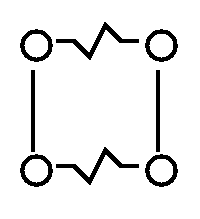
\includegraphics{pictures/1_Type1_1.eps}}
		\hspace{-4pt} 
		\resizebox{45px}{45px}{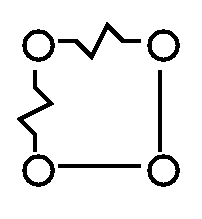
\includegraphics{pictures/1_Type1_2.eps}}
		\caption{Плакеты 1-го типа}
		\label{fig:Type1} 
	\end{minipage}
	\hspace{5pt} 
	\begin{minipage}{0.3\textwidth}
		\centering
		\resizebox{45px}{45px}{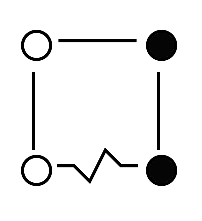
\includegraphics{pictures/1_Type2_1.eps}}
		\hspace{-2pt} 
		\resizebox{45px}{45px}{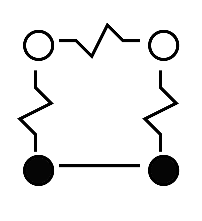
\includegraphics{pictures/1_Type2_2.eps}}
		\caption{Плакеты 2-го типа}
		\label{fig:Type2}
	\end{minipage}
	\hspace{5pt}
	\begin{minipage}{0.3\textwidth}
		\centering
		\resizebox{45px}{45px}{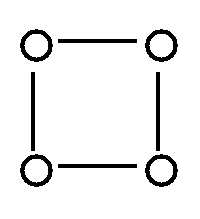
\includegraphics{pictures/1_Type3_1.eps}}
		\hspace{-4pt} 
		\resizebox{45px}{45px}{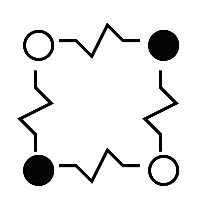
\includegraphics{pictures/1_Type3_2.eps}}
		\caption{Плакеты 3-го типа}
		\label{fig:Type3}
	\end{minipage}
\end{figure}


Всего в рассмотренных выше плакетах существует $2^4$ конфигураций.
Установлено, что фрустрация (возбуждение или положительная энергия обменного взаимодействия между $ij$-парой спинов) в основном состоянии обязательно появляется в плакетах 2-го типа, причём фрустрированной парой может быть любая пара спинов. Далее в центре таких плакетов будет размещаться знак $"+"$.

\section{Комбинаторика плакетов}

Если система состоит из двух плакетов 2-го типа, например, как показано на рисунке \ref{fig:Type2_32}, то для минимизации энергии фрустрированная пара будет расположена на пересечении плакетов, вне зависимости от расположения связей. 

\begin{figure}[H]
	\centering
	\begin{minipage}{0.3\textwidth}
		\centering
		\resizebox{90px}{60px}{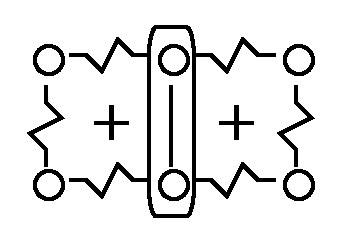
\includegraphics{pictures/1_Type2_3x2.eps}}
		\label{fig:Type2_3x2}
	\end{minipage}
	\hspace{20pt} 
	\begin{minipage}{0.3\textwidth}
		\centering
		\resizebox{90px}{60px}{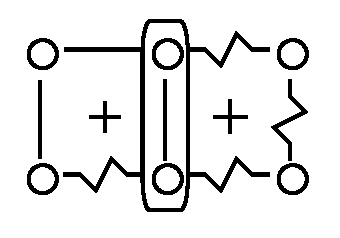
\includegraphics{pictures/1_Type2_3x2_2.eps}}
		\label{fig:Type2_3x2_2}
	\end{minipage}
	\caption{Системы состоящие из двух плакетов 2-го типа}
	\label{fig:Type2_32}
\end{figure}


Если известно, где расположена фрустрированная пара спинов, можно найти основное состояние системы. Таким образом, энергия основного состояния для систем на рисунке \ref{fig:Type2_32} будет $E_{gs}=-5$. Спиновый избыток основного состояния $M_{gs}=0$ для системы слева и $M_{gs}=\pm 2$ для системы справа.

Также стоит отметить, что на расположение фрустрации в таких системах  не влияют другие плакеты, находящиеся вокруг.

\begin{figure}[H]
	\centering
	\resizebox{100px}{70px}{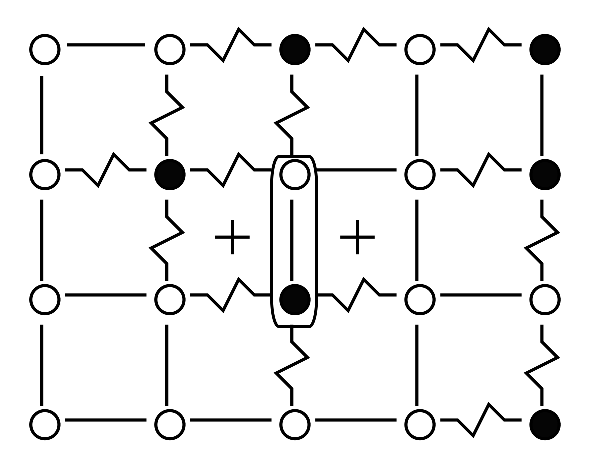
\includegraphics{pictures/1_Type2_5x4.eps}}
	\caption{Система из 20 спинов с двумя плакетами 2-го типа в центре}
	\label{fig:Type2_5x4}
\end{figure}

На рисунке \eqref{fig:Type2_5x4} представлена система из двадцати спинов, в центре которой находятся два плакета 2-го типа, имеющие общую пару спинов. Исходя из предыдущего примера, данная система должна обладать одной фрустрированной парой отмеченной на рисунке. Полный перебор состояний подтверждает, что в данной системе есть два основных состояния ($E_{gs}=-29$, $M_{gs}=\pm 8$), а фрустрация действительно расположена так как на рисунке.

\section{Плакеты в больших системах}

На рисунках \ref{fig:4x4.1} изображена система, где в центре решетки находится плакет 2-го типа. Так как плакет является одиночным то какую бы пару в нём мы не выбрали фрустрированной она будет также принадлежать соседнему плакету, не относящемуся ко 2-му типу. А так как в плакетах 1-го и 3-го типа не может быть одна фрустрированная пара, там будет присутствовать вторая фрустрация, причём таким образом чтобы не относиться к другим плакетам то есть с краю решётки. Данная система имеет 8 основных состояний ($E_{gs}=-20$, $M_{gs}=\pm 2, \pm 6, \pm 10$). Полный перебор подтверждает что в основных состояниях фрустрации расположены между плакетом 2-го типа и краем решётки.

\begin{figure}[htbp]
	\centering
	\begin{tabular}{cc}
		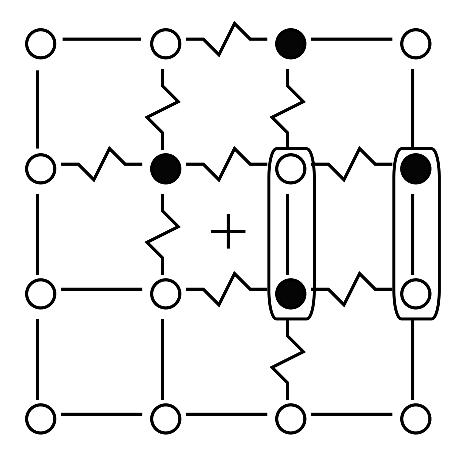
\includegraphics[width=0.2\textwidth]{pictures/1_Cl1_Type_gs1.eps}  \hspace{0.03\textwidth}
		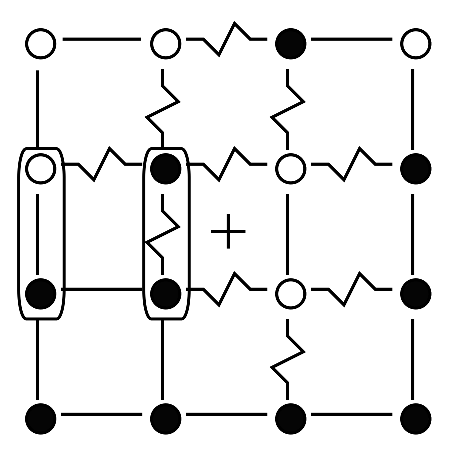
\includegraphics[width=0.2\textwidth]{pictures/1_Cl1_Type_gs2.eps} 
		\hspace{0.03\textwidth}
		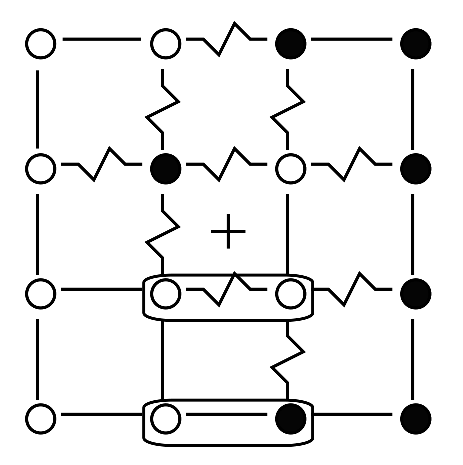
\includegraphics[width=0.2\textwidth]{pictures/1_Cl1_Type_gs3.eps}  \hspace{0.03\textwidth}
		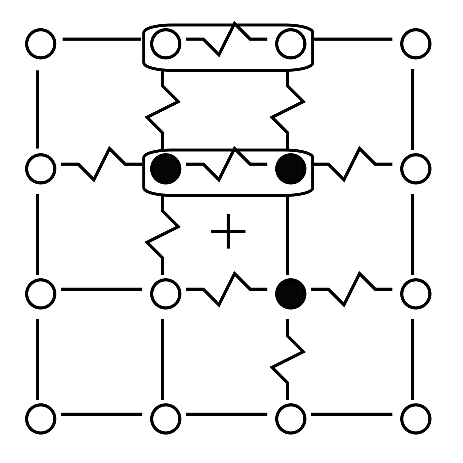
\includegraphics[width=0.2\textwidth]{pictures/1_Cl1_Type_gs4.eps} \\ 
	\end{tabular}
	\caption{Система из 16 спинов. Фрустрированные в основном состоянии пары обведены.}
	\label{fig:4x4.1}
\end{figure}

Если в системе два не пересекающиеся плакета 2-го типа \ref{fig:4x7} ($E_{gs}=-33$, $M_{gs}=0$), то возможна такая ситуация, что системе энергетически выгоднее, чтобы фрустрации находились между плакетами. 

\begin{figure}[H]
	\centering
	\resizebox{150px}{75px}{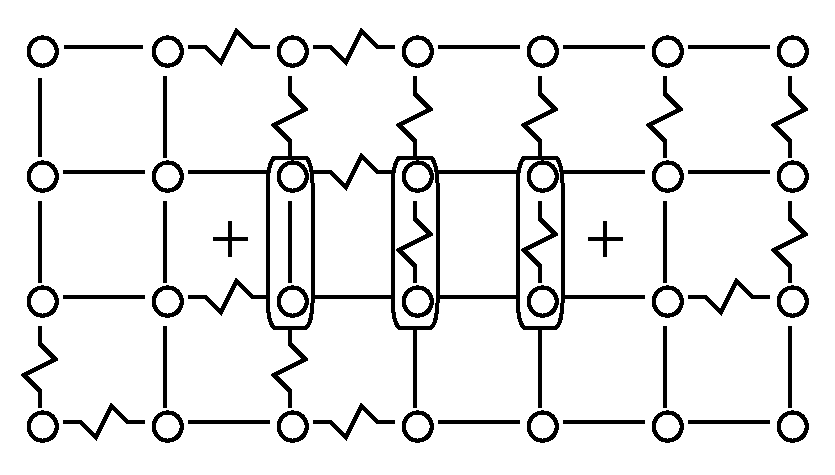
\includegraphics{pictures/1_Cl7x4_Type2.eps}}
	\caption{Система, обладающая двумя не пересекающимися плакетами 2-го типа}
	\label{fig:4x7}
\end{figure}

Также стоит рассмотреть случай, когда два плакета 2-го типа имеют лишь один общий спин \ref{fig:5x5.22F}. В этом случае также как и в предыдущем фрустрации в основном состоянии будут находиться между плакетами 2-го типа. Разница лишь в том, что один спин будет входить сразу в две фрустрированные пары.

\begin{figure}[H]
	\centering
	\begin{tabular}{cc}
		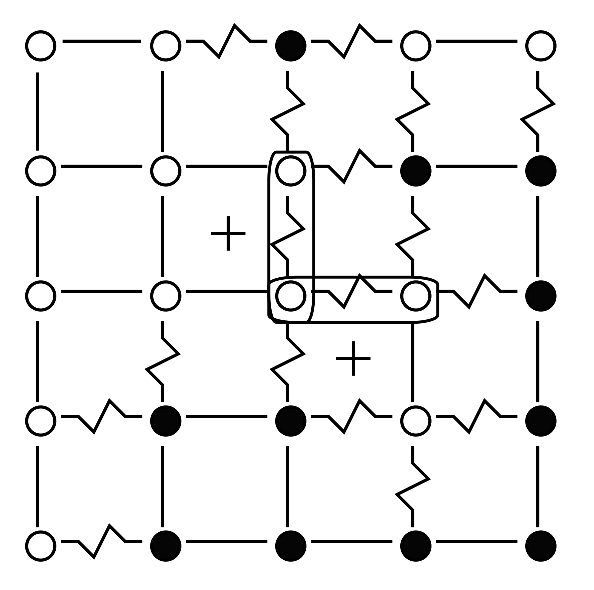
\includegraphics[width=0.25\textwidth]{pictures/1_Cl5x5_Type2_gs1.eps} & \hspace{0.05\textwidth}
		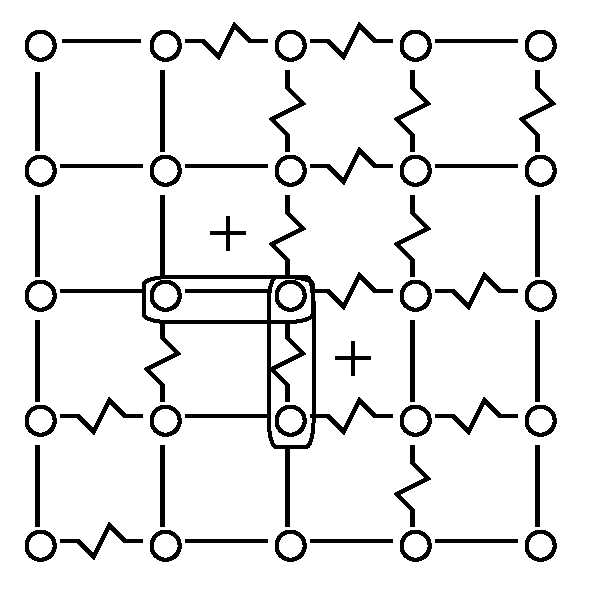
\includegraphics[width=0.25\textwidth]{pictures/1_Cl5x5_Type2_gs2.eps} 
	\end{tabular}
	\caption{Система из 25 спинов, в которой отмечены фрустрации в основных состояниях.}
	\label{fig:5x5.22F}
\end{figure}

\section{Кратность вырождения основного состояния}

На основе рассмотренных примеров можно сделать несколько выводов: \\
1. Плакеты 2-го типа являются единственной причиной возникновения фрустраций в основном состоянии.\\
2. В основном состоянии фрустрации расположены между плакетами 2-го типа или между плакетом и краем решётки в зависимости от расстояний.

Далее исходя из выводов был сформулирован алгоритм по поиску всех основных состояний путём комбинирования разбиений плакетов 2-го типа на пары.

Рассмотрим работу алгоритма на примере решётки состоящей из 64 спинов \ref{fig:cell64_J72_5}.

\begin{figure}[H]
	\centering
	\resizebox{150px}{150px}{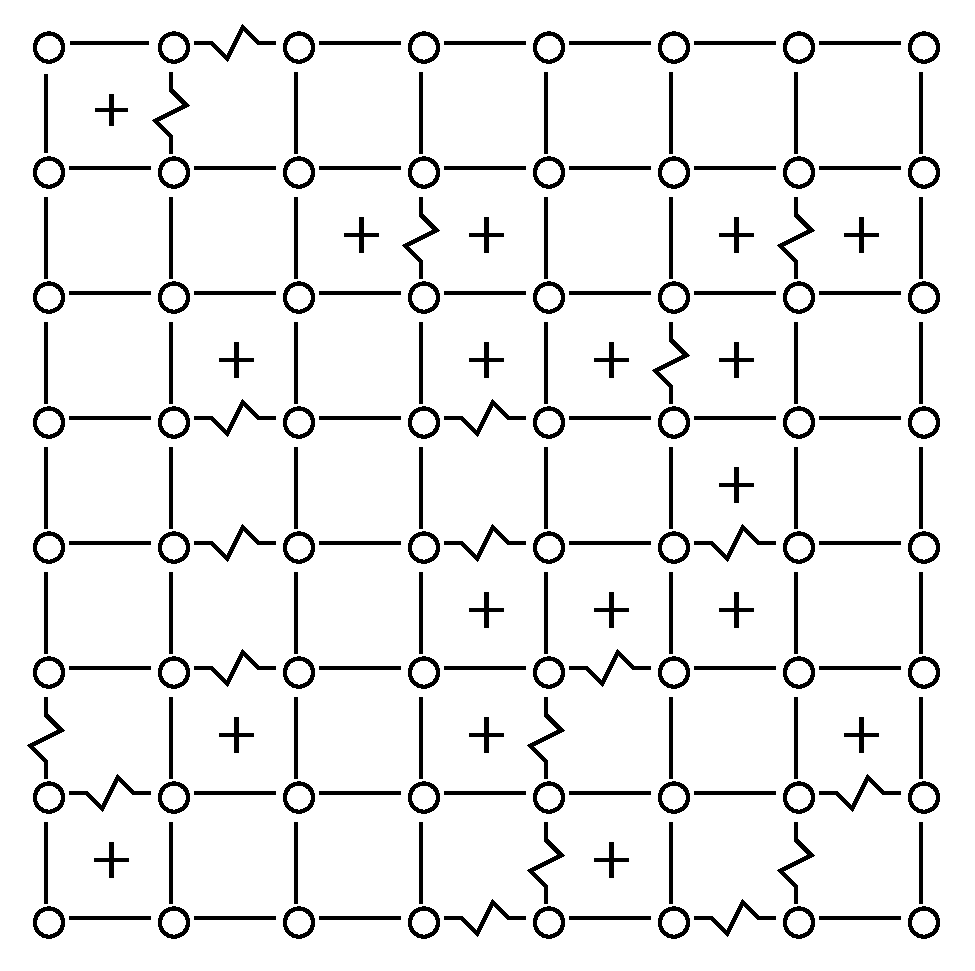
\includegraphics{pictures/0_cell64_J72_5.eps}}
	\caption{Пример решётки из 64 спинов}
	\label{fig:cell64_J72_5}
\end{figure}

Сначала каждому плакету присваиваются координаты $x$ и $y$. Далее происходит комбинирование разбиений плакетов второго типа по парам. Рассматриваются случаи когда фрустрации возникают между каждой парой плакетов и когда размещение возбуждений происходит между плакетом и краем решётки. Число фрустраций между $i,j$-той парой плакетов определяется как $\left|x_i-x_j\right|+\left|y_i-y_j\right|$,  число фрустраций, возникающее от плакета 2-го типа до ближайшего края решетки определяется как $R_{ij}+1$, где i - номер плакета 2-го типа, j - номер ближайшего плакета находящегося на краю решётки, $R_{ij}$ - расстояние между ними. После перебора рассматриваются комбинации, которые по подсчётам обладают минимальным числом фрустраций. Несколько из них представлены на рисунке \ref{fig:12PS_cell64_J72_5}.

\begin{figure}[H]
	\centering
	\begin{tabular}{cc}
		\resizebox{150px}{150px}{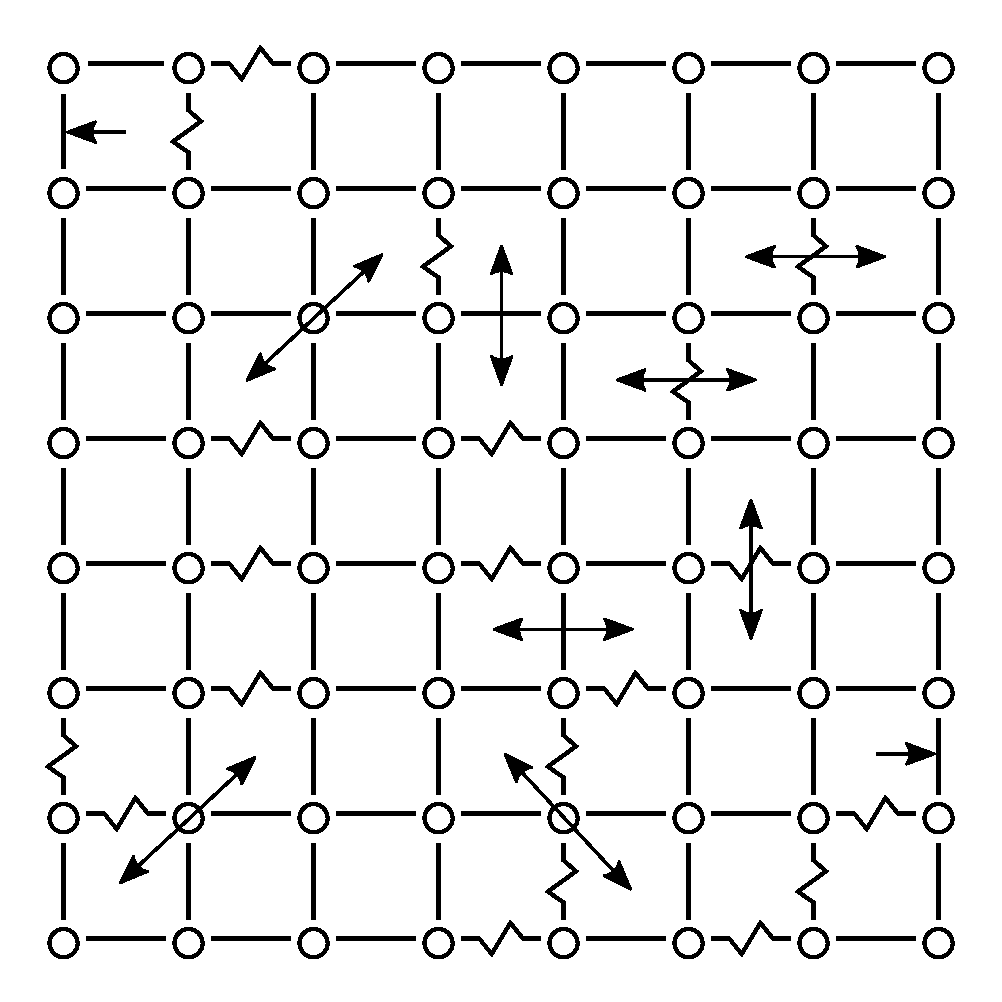
\includegraphics[width=0.25\textwidth]{pictures/1PS_cell64_J72_5.eps}} & \hspace{0.05\textwidth}
			\resizebox{150px}{150px}{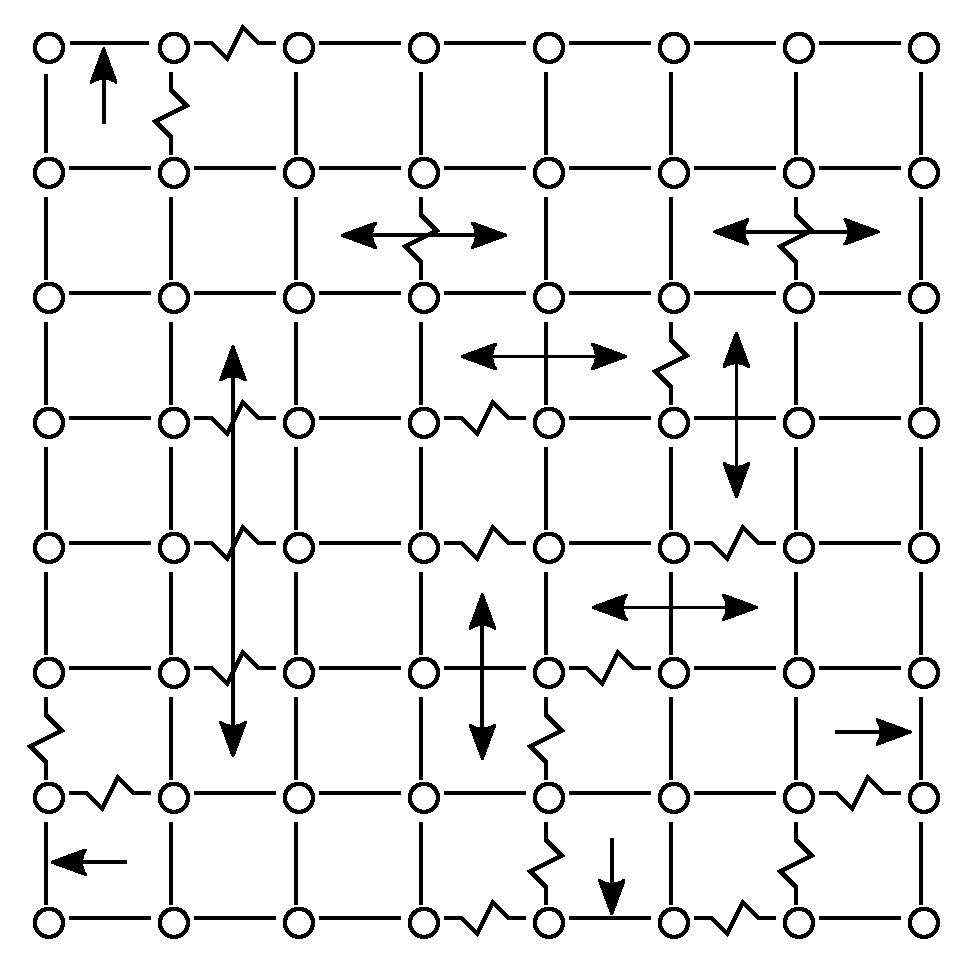
\includegraphics[width=0.25\textwidth]{pictures/2PS_cell64_J72_5.eps}} 
	\end{tabular}
	\caption{Комбинации плакетов 2-го типа обладающих минимальным числом фрустраций}
	\label{fig:12PS_cell64_J72_5}
\end{figure}

Далее на основании полученных комбинаций отмечаются как фрустрации пары спинов находящиеся между плакетами \ref{fig:12F_cell64_J72_5}.

\begin{figure}[H]
	\centering
	\begin{tabular}{cc}
		\resizebox{150px}{150px}{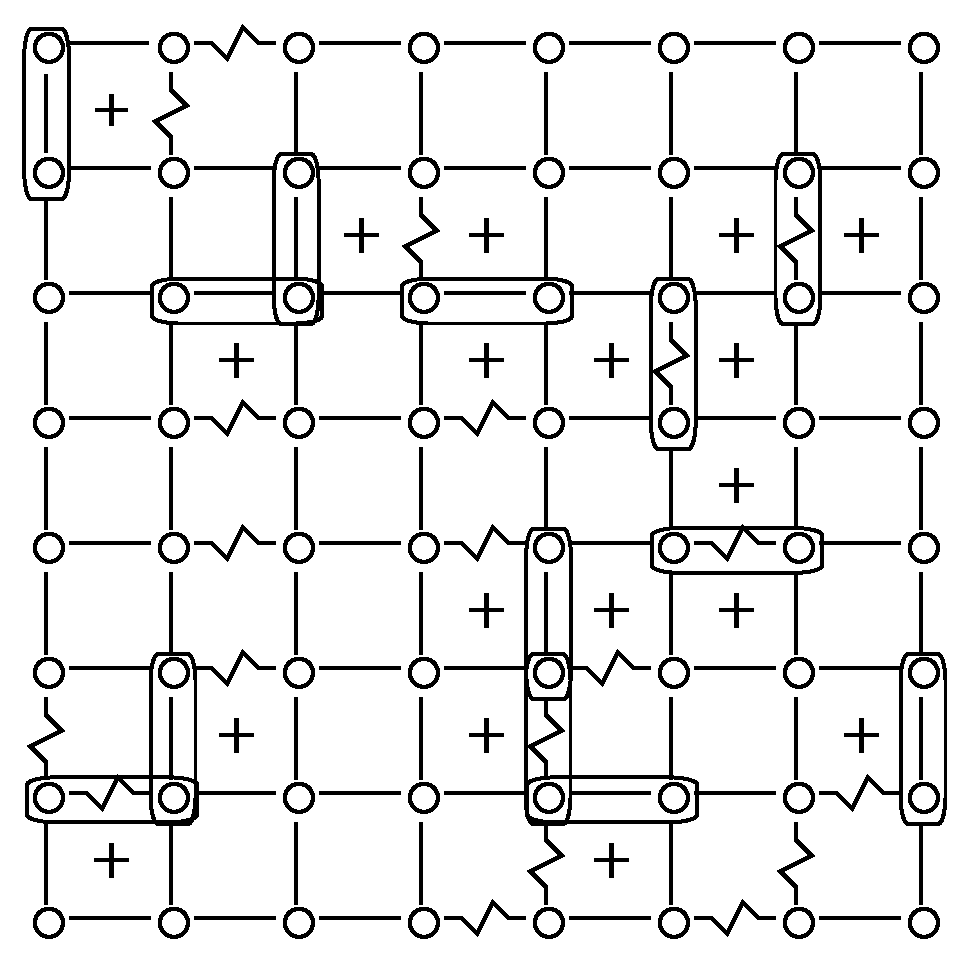
\includegraphics[width=0.25\textwidth]{pictures/1F_cell64_J72_5.eps}} & \hspace{0.05\textwidth}
		\resizebox{150px}{150px}{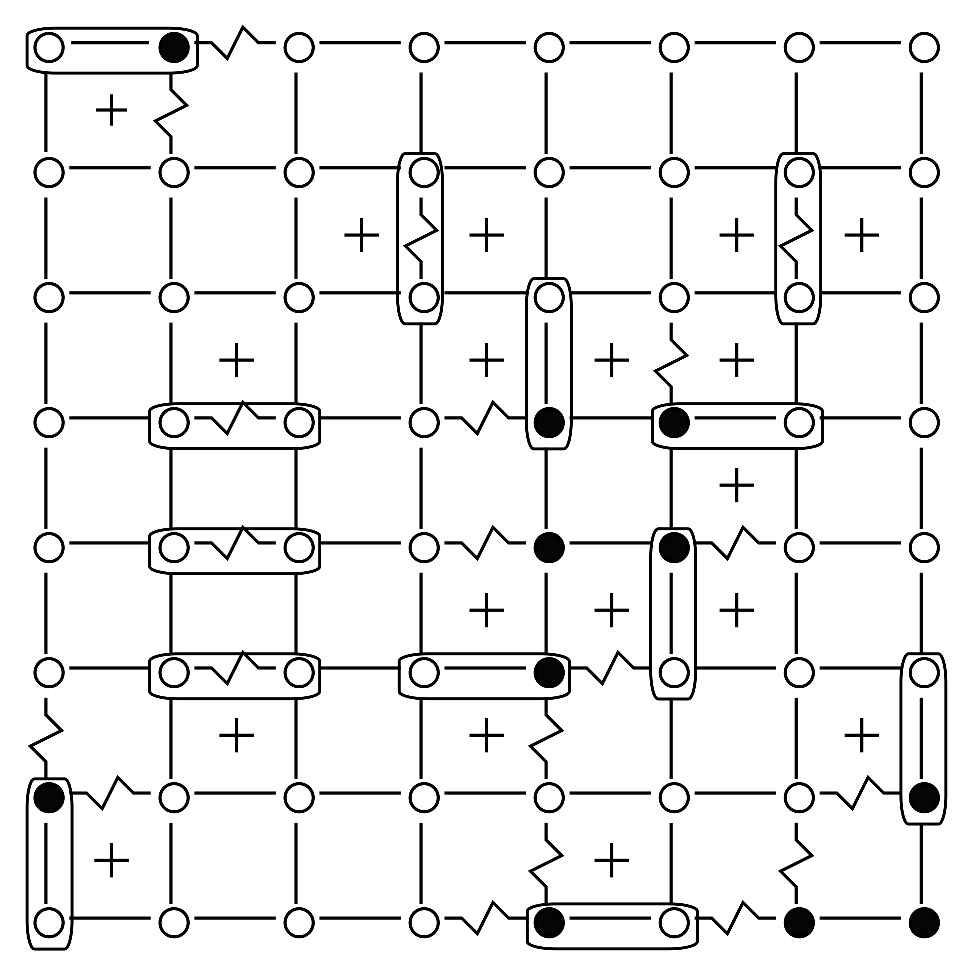
\includegraphics[width=0.25\textwidth]{pictures/2F_cell64_J72_5.eps}} 
	\end{tabular}
	\caption{Фрустрации в основных состояниях решётки}
	\label{fig:12F_cell64_J72_5}
\end{figure}

Точно зная где в основных состояний расположены фрустрации можно расставлять значения спинов по порядку так чтобы они удовлетворяли все связи и давали положительную энергию во фрустрированных парах и отрицательную в не фрустрированных. 

Всего для данной решётки были получены 124 основных состояния с энергией $E_{gs}=-86$ и спиновым избытком от $\pm 18$ до $\pm 42$. Данное решение полностью совпадает с алгоритмом вычисления плотности состояний \ref{alg:addititional_algorithm} .

Такая высока кратность вырождения основного состояния обусловлена несколькими причинами:\\
1. Различные комбинации плакетов 2-го типа могут давать одинаковое количество фрустраций, как показано в предыдущем примере \ref{fig:12PS_cell64_J72_5}.\\
2. Может существовать несколько расстановок фрустраций между плакетами если их координаты $x,y$ обе различаются \ref{fig:5x5.22F}.\\
3. Для плакета возбуждения которого находятся между краем решётки может быть несколько краёв находящихся на одинаковом расстоянии \ref{fig:4x4.1}.\\


\section{Решение исчерпывающим перечислением}

Модель спинового стекла Эдвардса-Андерсона представляет собой плоскую решетку Изинга:

\begin{equation}
	E = -\sum J_{ij} S_i S_j + h \sum S_i.
	\label{eq:ising_energy}
\end{equation}
Это приводит к конкурирующим антиферромагнитным (при $J_{ij}=-1$) и ферромагнитным (при $J_{ij}=+1$) взаимодействиям. В нашей модели энергия обменного взаимодействия не зависит от расстояния между взаимодействующими спинами. Однако, знакопеременный характер обменных интегралов $J_{ij}$ может быть связан с искажениями в размещении взаимодействующих атомов на решетке, осцилляциями электронной плотности.

Рассмотрим одномерную цепочку из трёх спинов ($L=3$), взаимодействующих ферромагнитно.  В этом случае $J_{ij}=+1$.  Обозначим $\beta = (kT)^{-1}$.  Статистическая сумма принимает вид:

\begin{equation}
	Z_3 = e^{3\beta - 3\beta h} + 3e^{\beta - h - \beta} + 3e^{\beta h - \beta} + e^{3\beta + 3\beta h}.
	\label{eq:stat_3}
\end{equation}

Присоединим вторую цепочку параллельно первой. С учетом того, что у нас все взаимодействия ферромагнитные

\begin{equation}
	\label{eq:stat_3_un}
	\begin{alignedat}{2}
		Z_6 = Z_3 e^{\beta  h-\beta }+Z_3 e^{\beta  h-\beta }+Z_3 e^{\beta  h-\beta }+Z_3 e^{3 \beta +3 \beta  h}+ \\
		Z_3 e^{\beta  (-h)-\beta }+Z_3 e^{\beta  (-h)-\beta }+Z_3 e^{\beta  (-h)-\beta }+Z_3 e^{3 \beta -3 \beta  h}.
	\end{alignedat}
\end{equation}

В результате получаем статистическую сумму для решетки $3 \times 2$:

\begin{equation}
	\label{eq:stat_3_res}
	\begin{alignedat}{2}
		Z_6 = 6 e^{-5 \beta }+12 e^{-\beta }+2 e^{3 \beta }+e^{9 \beta -6 \beta  h}+6 e^{3 \beta -4 \beta  h}+6 e^{-3 \beta -2 \beta  h}+\\
		9 e^{\beta -2 \beta  h}+6 e^{2 \beta  h-3 \beta }+9 e^{\beta +2 \beta  h}+6 e^{3 \beta +4 \beta  h}+e^{9 \beta +6 \beta  h}.
	\end{alignedat}
\end{equation}

Алгоритм численного расчета  параметров статистической суммы (плотности состояний, вырождения или энтропии, энергии и спинового избытка состояний) тогда выглядит следующим образом \ref{alg:addititional_algorithm}:


\begin{algorithm}[H]
	\textbf{ВХОД:} Размер и геометрия решетки (количество и координаты спинов, граничные условия, число соседей), распределение обменных констант.\\
	\textbf{ВЫХОД:} Параметры статистической суммы, плотность состояний - (вырождение или энтропия, энергия и спиновый избыток).
	\begin{algorithmic}
		\STATE {Рассчитать плотность состояний для первой 1D цепочки}
		\FOR {Количество слоев в решетке\\}
		{
			\STATE {Рассчитать плотность состояний для присоединяемой 1D цепочки}
			\FOR {длина 1D цепи\\}
			{
				\STATE {Рассчитать плотность состояний для получившейся решетки}
			}
			\ENDFOR\\
		}
		\ENDFOR
	\end{algorithmic}
	\caption{Вычисление параметров статистической суммы методом присоединения 1D цепочек.}
	\label{alg:addititional_algorithm}
\end{algorithm}

В результате для квадратной решетки $L \times L=N$ сложность алгоритма полного перебора падает с $2^{N}$ до $L \cdot 2^L + (L - 1) \cdot 2^L$. Таким образом прирост производительности для решетки из 9-ти спинов составляет примерно 92\% и на 27 порядков для системы из 100 спинов.


\section{Энергия основного состояния}

Результаты решения задачи о вычислении энергии основного состояния спинового стекла в модели Эдвардса-Андресона приведены в таблице \ref{tab:Egs}. Из таблицы видно, что энергии основного состояния  имеют большой разброс.

\begin{table}[h]
	\begin{tabular}{|l|c|l|}
		\hline
		Method                                   & $E_{gs}$                                       & ссылка                                          \\ \hline
		Thouless-Anderson-Palmer (TAP) Approach & 0                                              & \cite{thouless1977solution}    \\ \hline
		Replica Method                            & $-2/\pi$                                       & \cite{sherrington1975solvable} \\ \hline
		Partition function                      & -0.5                                           & \cite{tanaka1980analytic}      \\ \hline
		Mean random field                       & $-1/\sqrt{2\pi}$                               & \cite{klein1976comparison}     \\ \hline
		Monte-Carlo                             & -0.76                                          & \cite{kirkpatrick1978infinite} \\ \hline
		Algorithm of Shraudorphs-Kamensky        & -1.33                                          & \cite{karandashev2019global}   \\ \hline
		Parallel Tempering   & -1.40193                                       & \cite{palmer1999ground}        \\ \hline
		Branch-and-Cut Algorithm              & -1.40197                         
		& \cite{campbell2004energy}      \\ \hline
		
		Parallel tempering Monte-Carlo  & -1.31479                                       & \cite{roma2009ground}          \\ \hline
		
		
		
	\end{tabular}
	\label{tab:Egs}
	\caption{Удельная энергия основного состояния}
\end{table}

В данной работе мы вычислили значения энергии основного состояния в модели Эдвардса-Андерсона точно с помощью исчерпывающего перечисления (алгоритм \ref{alg:addititional_algorithm}
) и с помощью описанного выше подхода. Для исследования основных состояний были взяты 2000 различных решёток спинового стекла. Линейный размер $L$ в образцах был от 8 до 32.
Для каждого размера рассматривались системы с различным чётным количеством плакетов 2-го типа (от 2 до 16) и для каждого количества плакетов было взято по 10 систем со случайной расстановкой плакетов 2-го типа внутри системы. Для исследования не  брались решётки с нечётным количеством плакетов 2-го типа так как тогда невозможно добиться одинакового количества отрицательных и положительных обменных интегралов в системе. 

Из графика \ref{fig:Egs_N_F} видно, что энергия основного состояния системы на один спин увеличивается с числом фрустрированных плакетов. Диапазон таких значений составляет -1.92578 ; -1.34375. Более низкое значение удельной энергии по сравнению с данными в таблице \ref{tab:Egs} обусловлено тем, что для данного исследования были взяты системы с небольшим количеством плакетов 2-го типа, что уменьшает количество фрустраций в основных состояниях.

\begin{figure}[H]
	\centering
	\resizebox{300px}{150px}{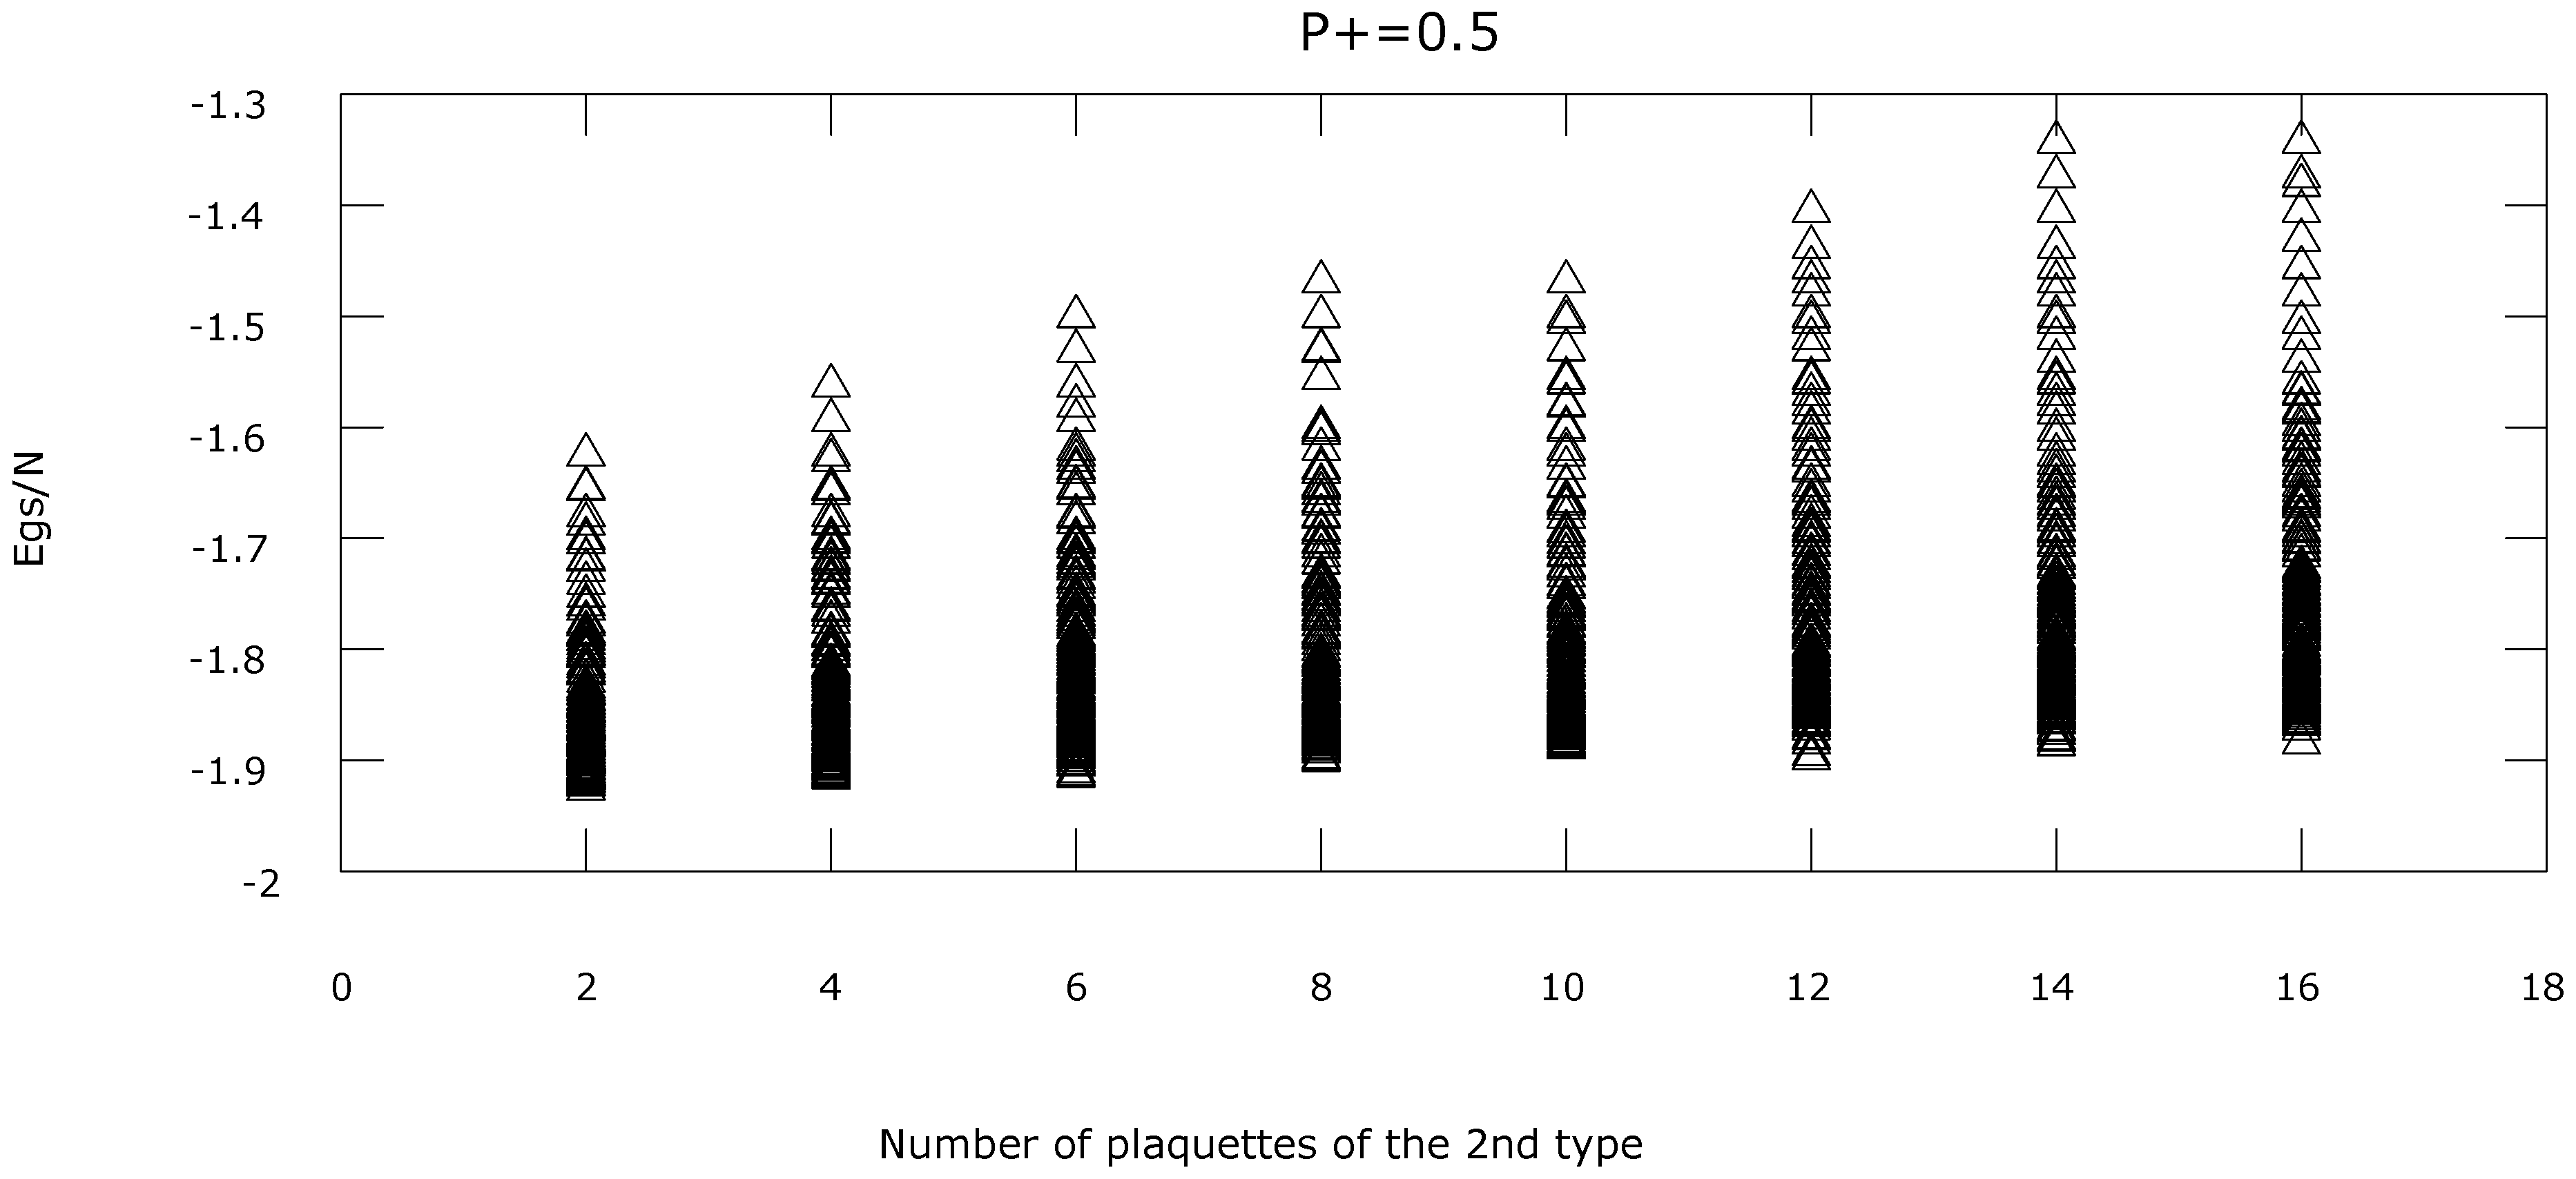
\includegraphics{pictures/Egs_N_F.eps}}
	\caption{Зависимость удельной энергии основного состояния на один спин от количества плакетов 2-го типа.}
	\label{fig:Egs_N_F}
\end{figure}

Из графика \ref{fig:Egs____N_F} видно, что с увеличением спинов в системе удельная энергия стремится к -2.

\begin{figure}[H]
	\centering
	\resizebox{300px}{150px}{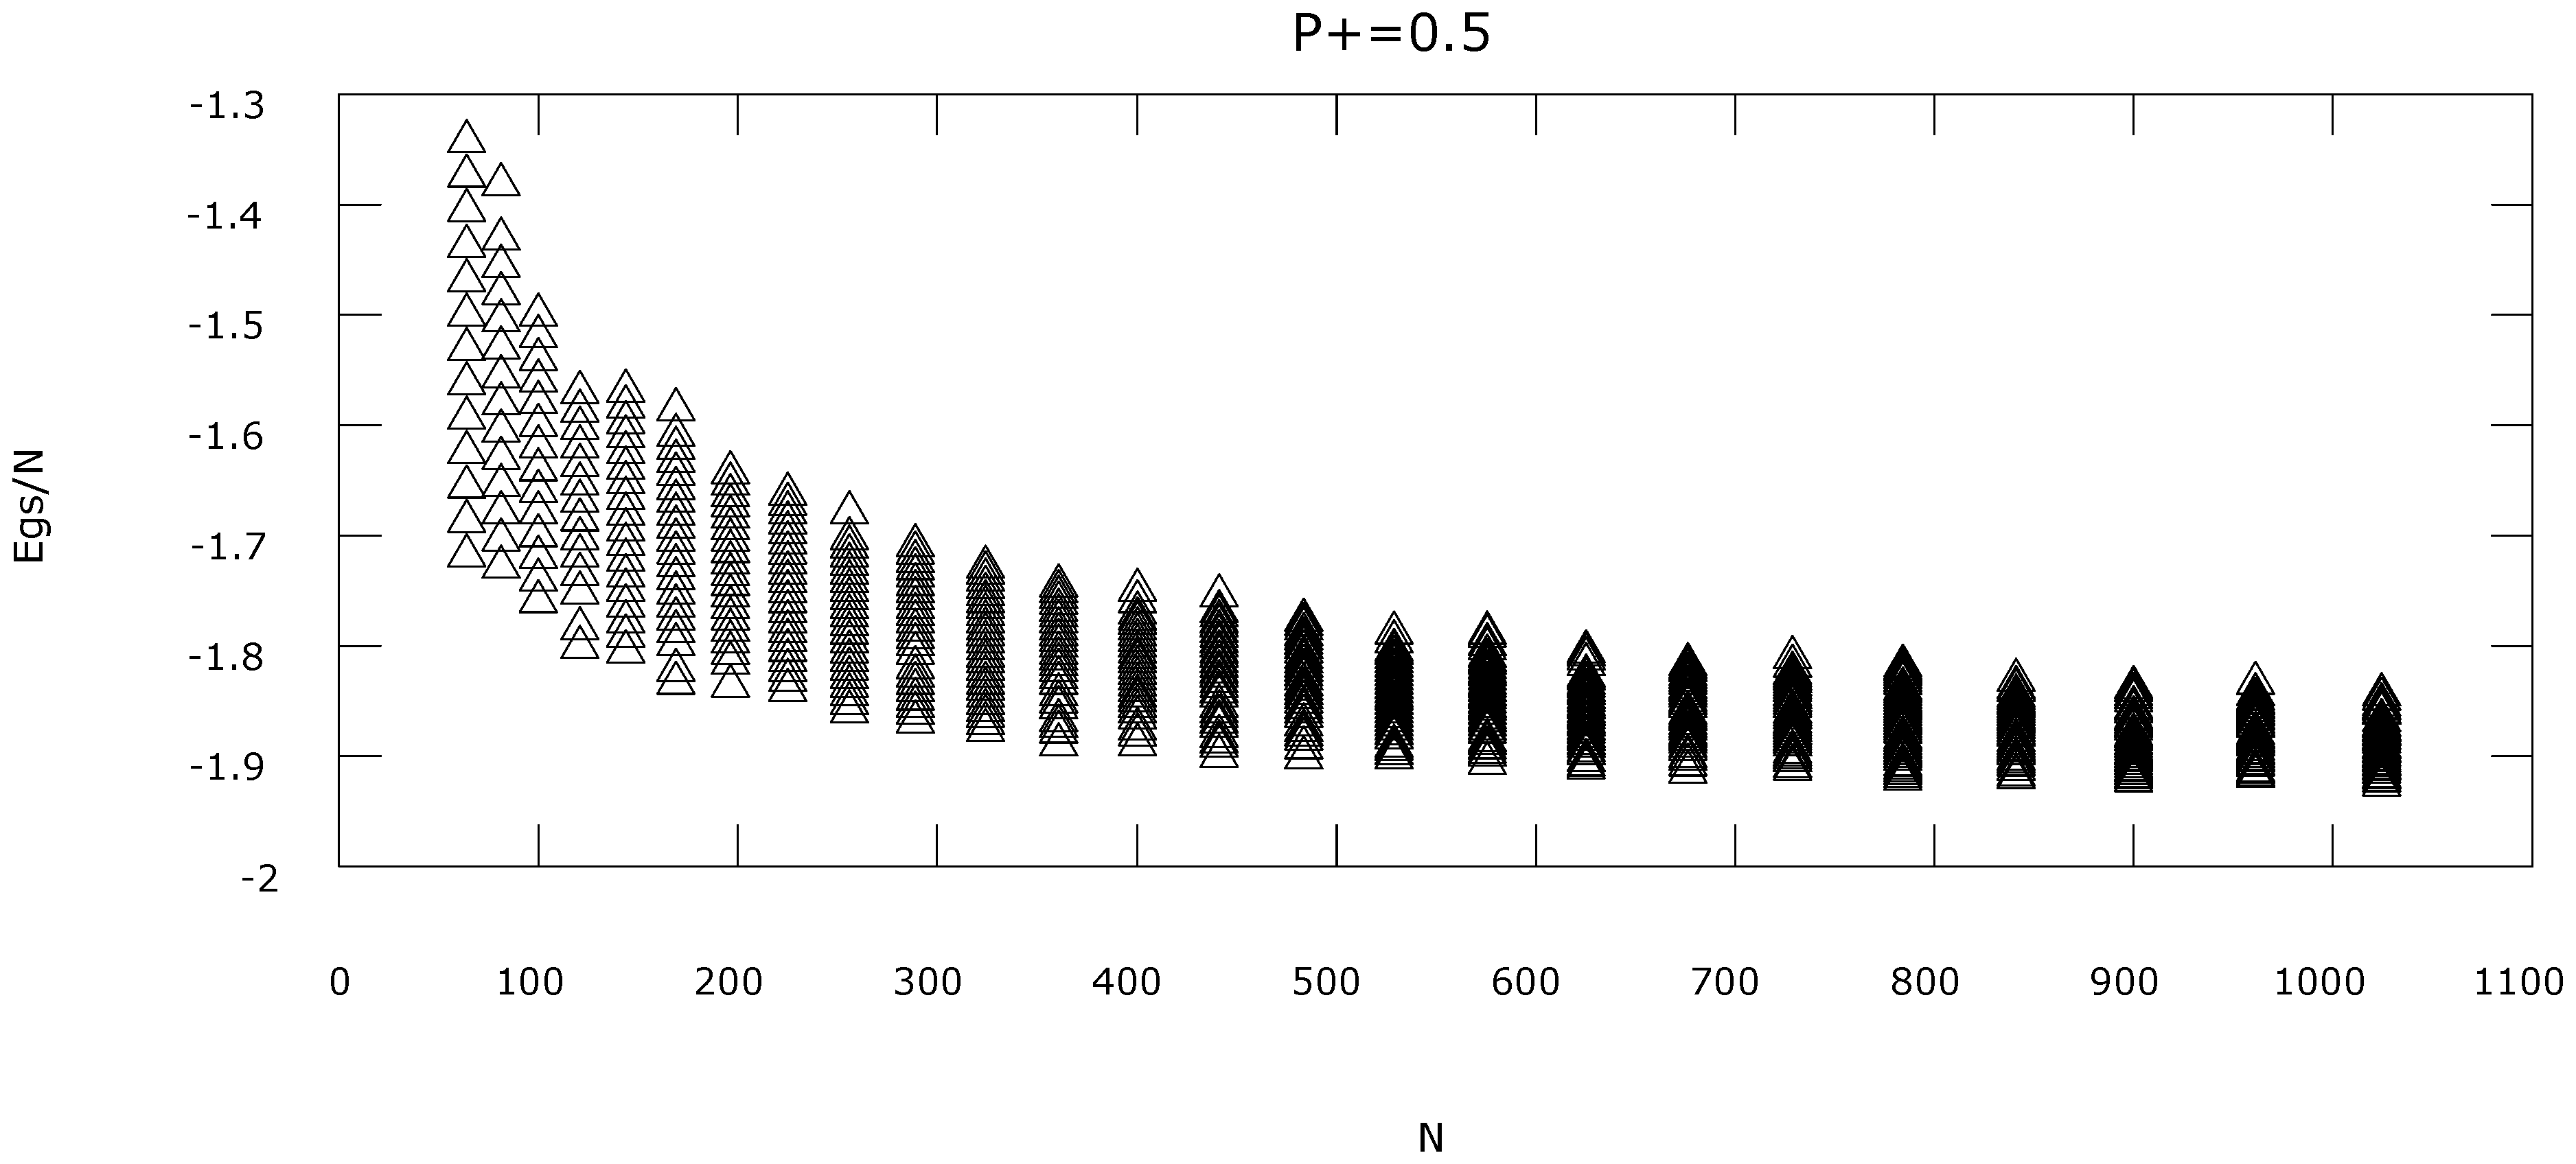
\includegraphics{pictures/Egs_N_N.eps}}
	\caption{Зависимость удельной энергии основного состояния от количества спинов}
	\label{fig:Egs____N_F}
\end{figure}



\section{Основное состояние во внешнем магнитном поле}



Во введении приведена таблица \ref{tab:Egs} со значениями энергии основного состояния спинового стекла. Мы создали несколько образцов спинового льда, один из них на рисунке (\ref{fig:cell_SI_SG_64}) слева. Вычисления показывают, что энергия основного состояния на один спин при $P_+ = 0.5$ и отсутствии воздействия внешнего магнитного поля составила -0.97, при этом удельная энергия основного состояния спинового стекла в модели Эдвардса-Андерсона составила -1.28. Под спиновым льдом обычно понимается магнетики с периодичностью в обменных взаимодействиях \cite{peretyatko2017interplay, otsuka2018husimi, andriushchenko2019large, shevchenko2017effect, kato2022flux}. 

\begin{figure}[H]
	\begin{minipage}[h]{0.3\linewidth}
		\centering(a)
		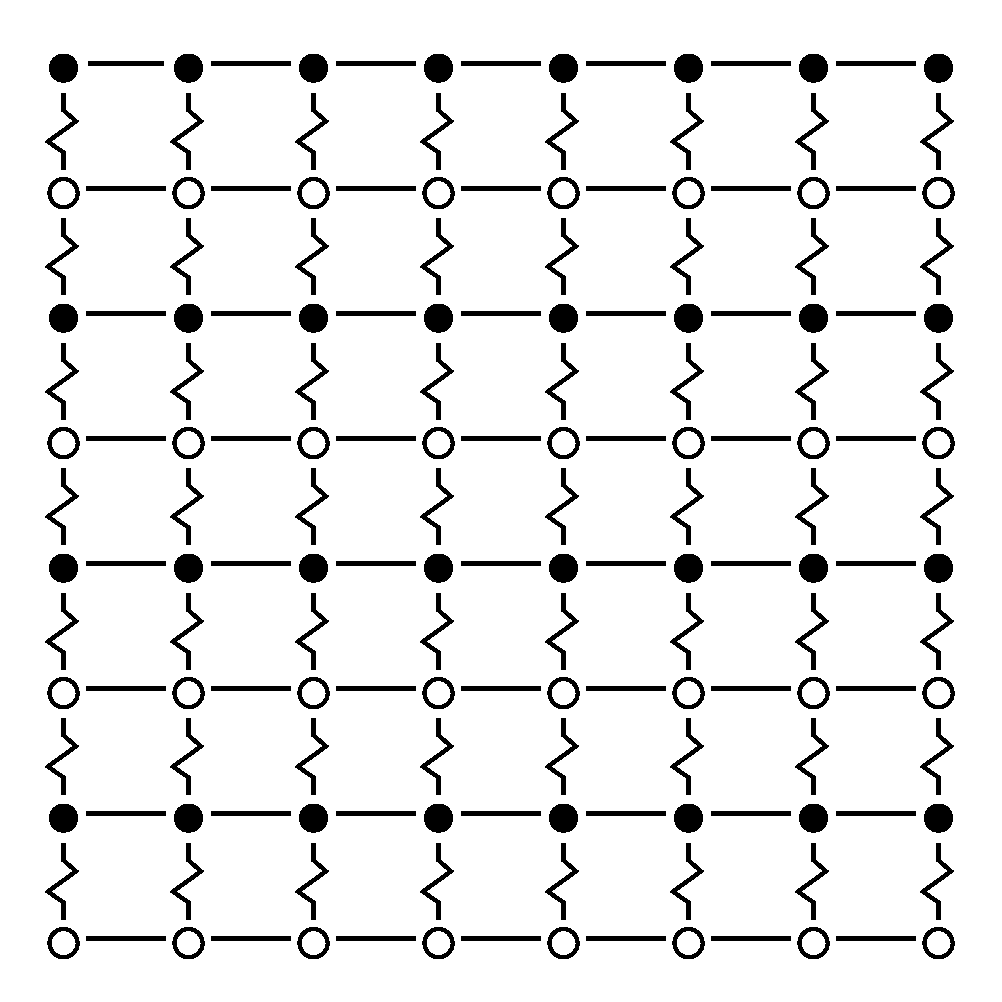
\includegraphics[width=1\linewidth]{pictures/SI_64_J0_1}
	\end{minipage}
	\hfill
	\begin{minipage}[h]{0.3\linewidth}
		\centering(b)
		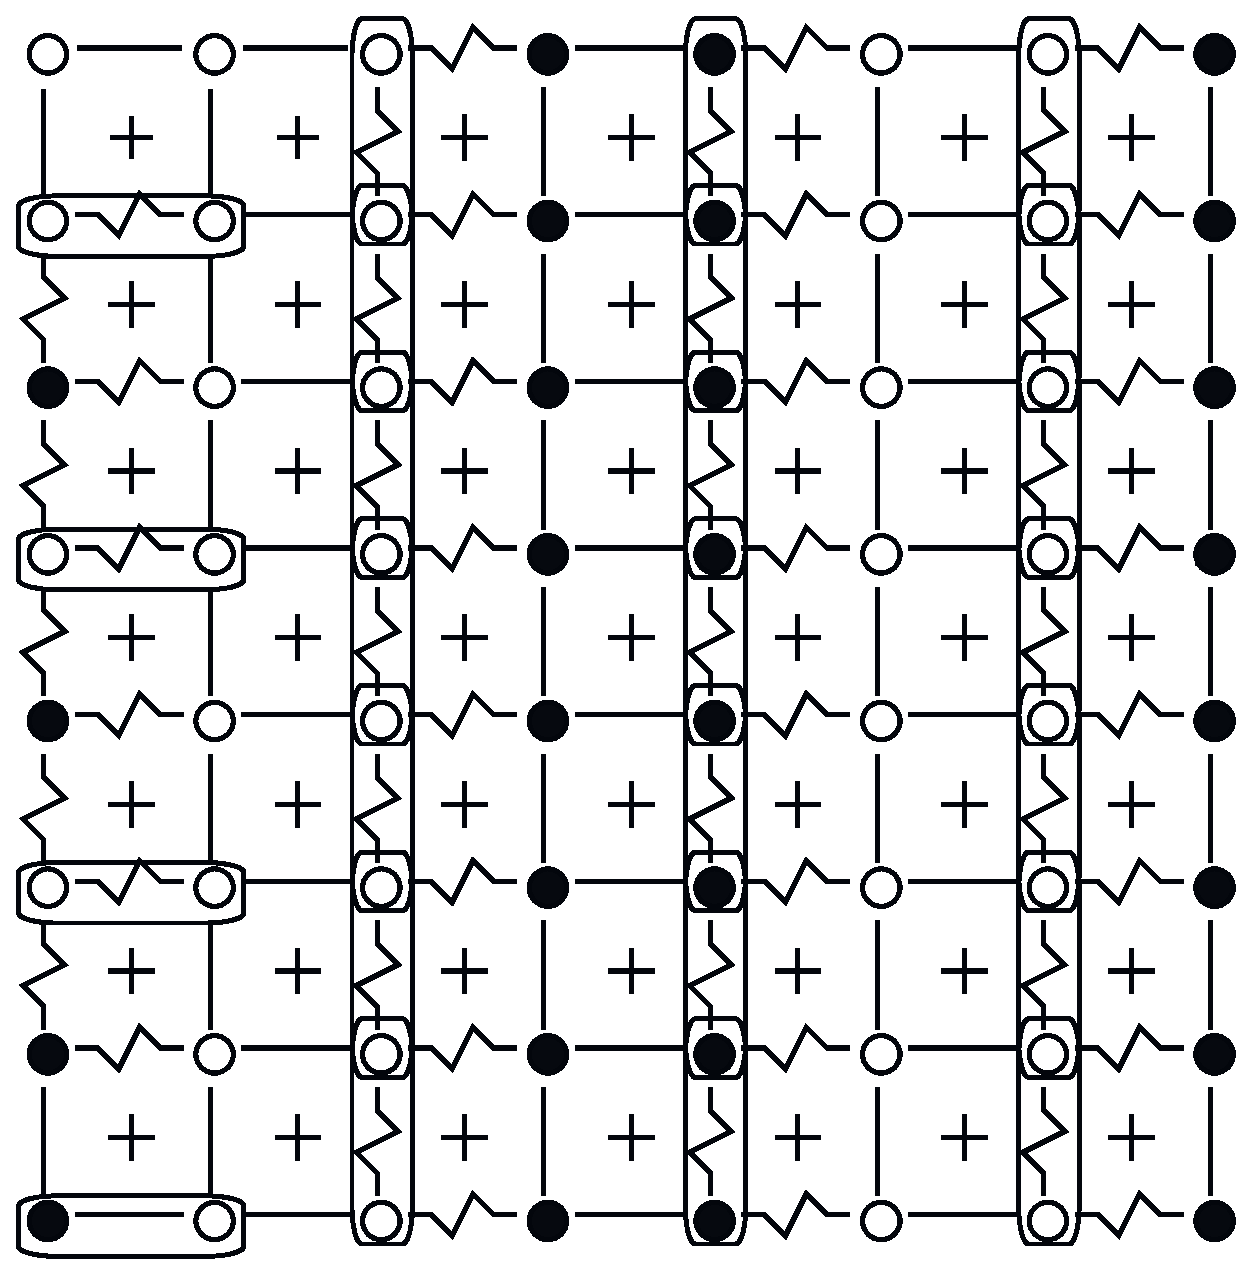
\includegraphics[width=1\linewidth]{pictures/SI_64_J0}
	\end{minipage}
	\hfill
	\begin{minipage}[h]{0.3\linewidth}
		\centering(c)
		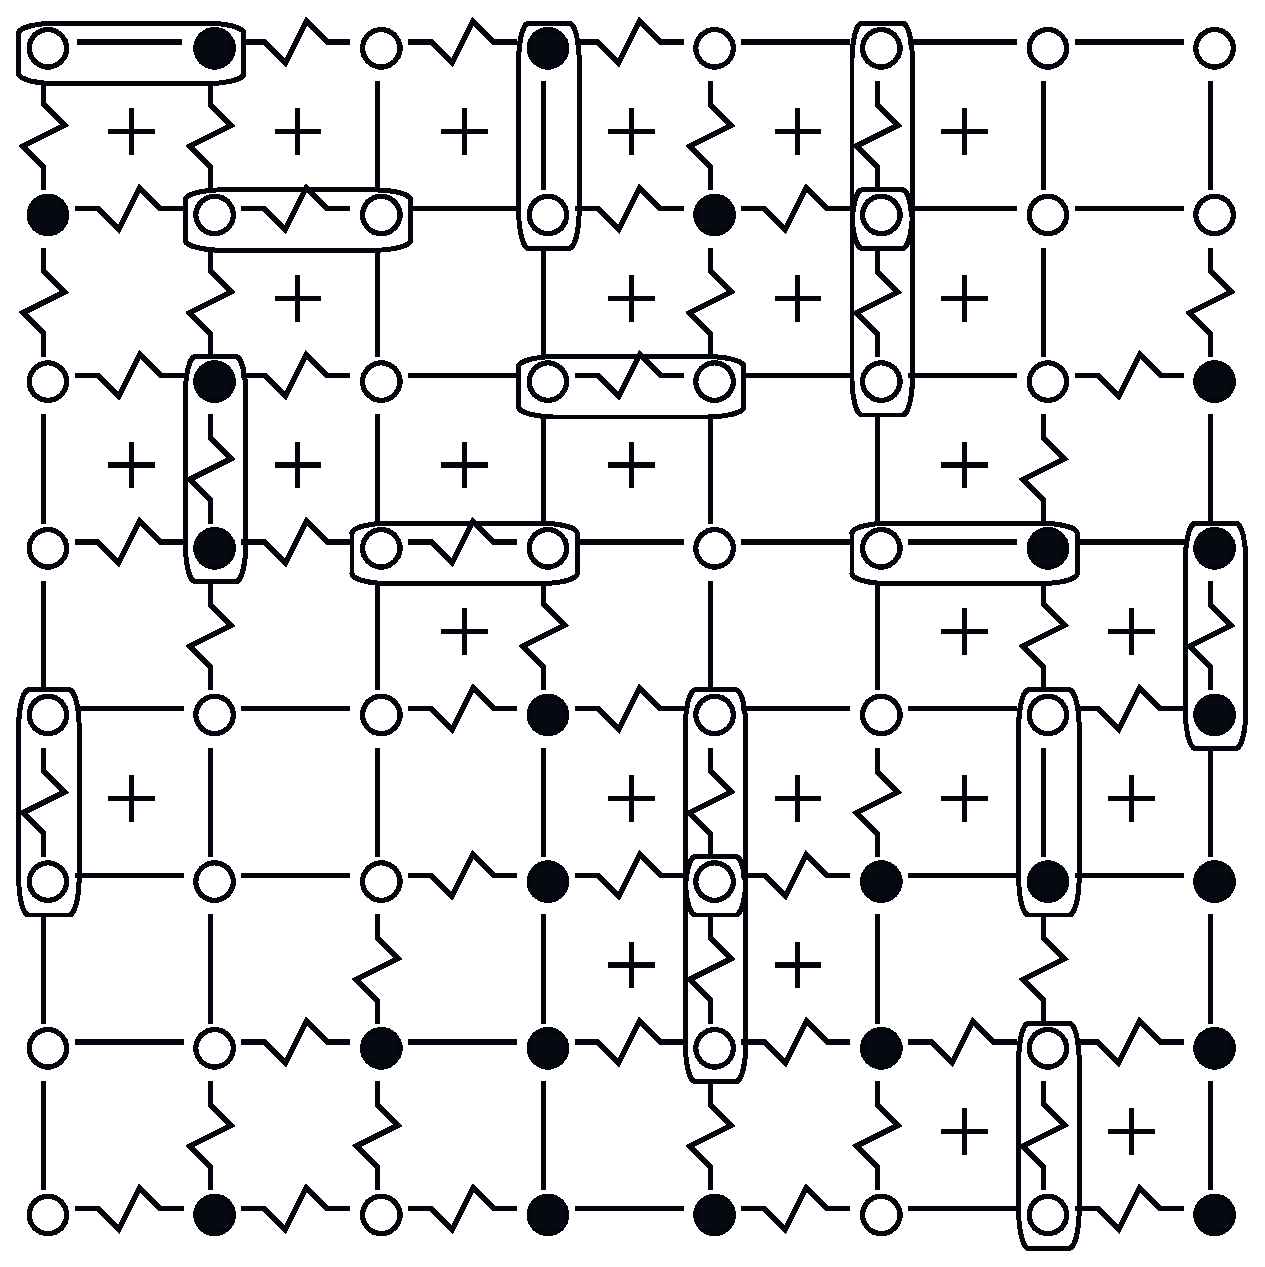
\includegraphics[width=1\linewidth]{pictures/SG_64_J0}
	\end{minipage}

	\caption{Спиновый лед (a,b) и спиновое стекло (c), 64 спина, $P_+ = 0.5$}
	\label{fig:cell_SI_SG_64}

\end{figure}




\begin{figure}[H]
	\begin{minipage}[h]{0.45\linewidth}
		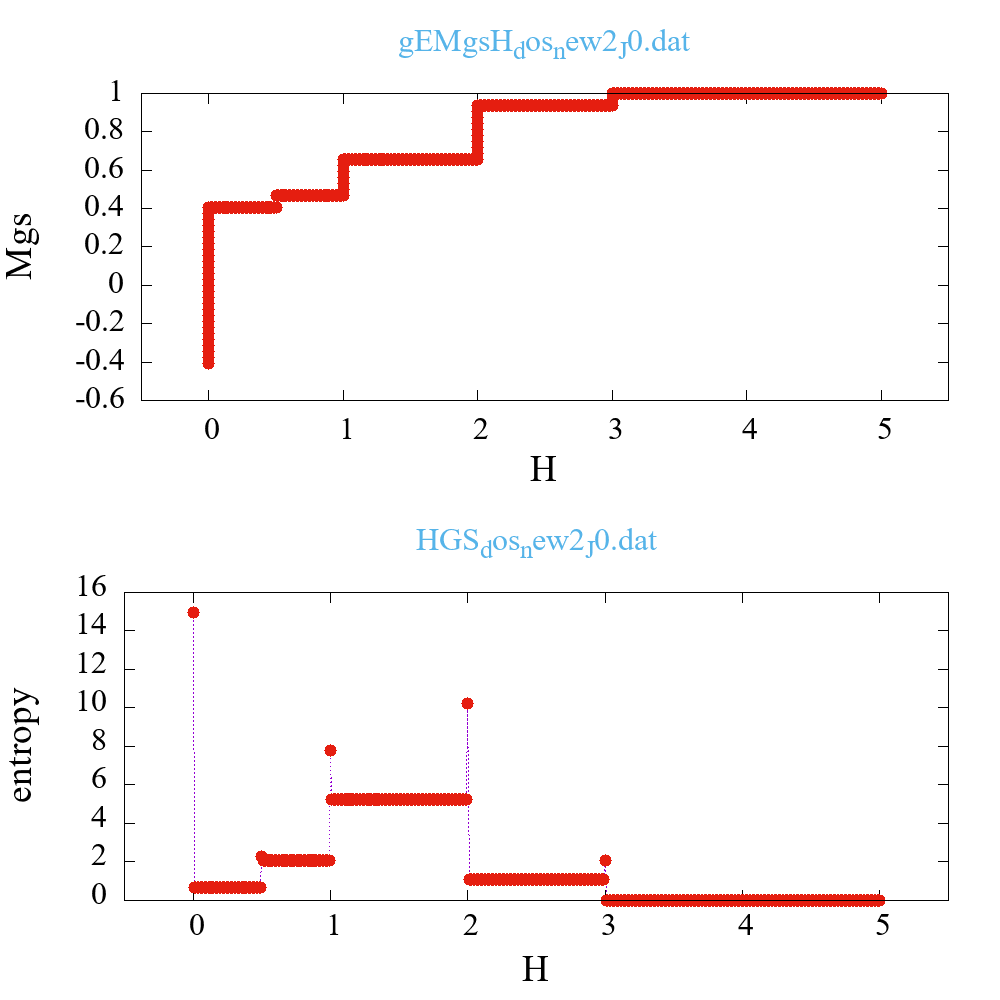
\includegraphics[width=1\linewidth]{pictures/_multiplot_SI64_J0.png}
	\end{minipage}
	\hfill
	\begin{minipage}[h]{0.45\linewidth}
		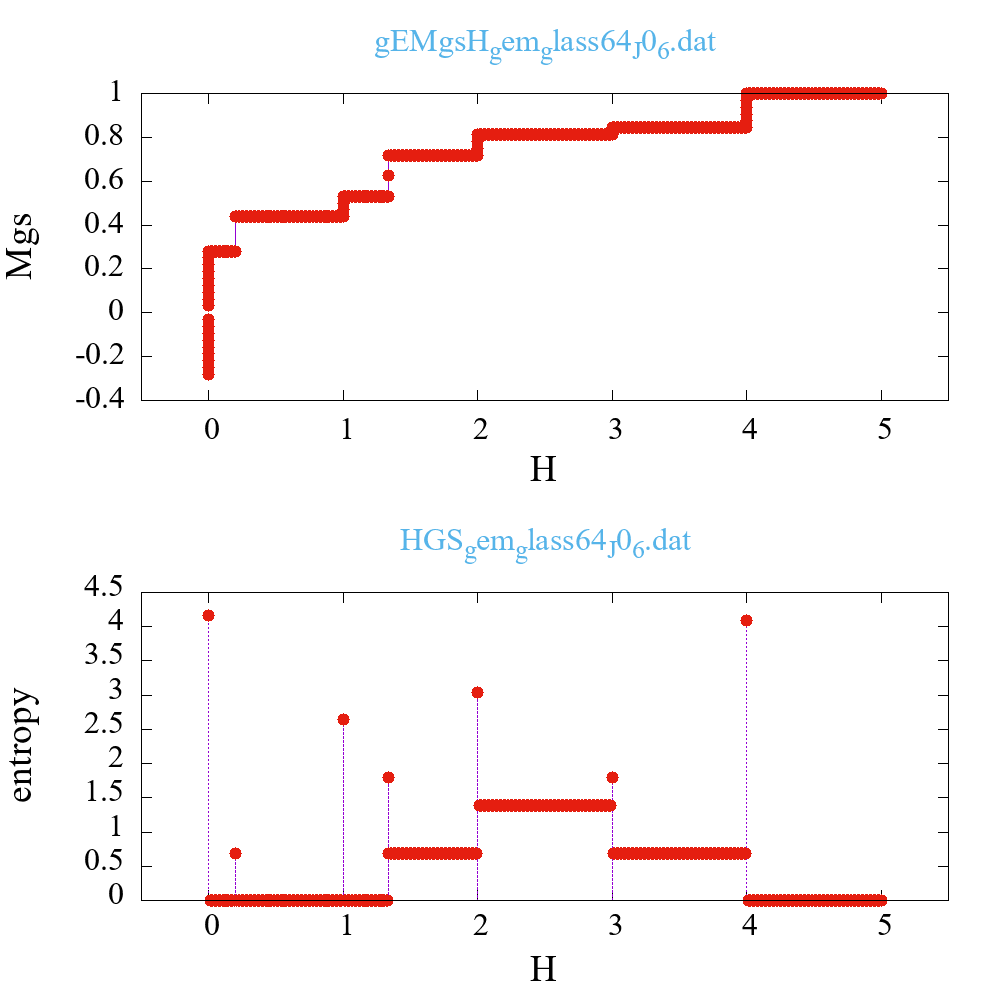
\includegraphics[width=1\linewidth]{pictures/_multiplot_SG64_J0.png}
	\end{minipage}
	\caption{Спиновый лед (слева) и спиновое стекло (справа), 64 спина, $P_+ = 0.5$}
	\label{fig:_multiplot_SI_SG_64}
\end{figure}


Методом полного перебора для образцов спинового льда и спинового стекла, представленных на рис. \ref{fig:cell_SI_SG_64}, были построены плотности распределения состояний в зависимости от критических значений внешнего магнитного поля (рис. \ref{fig:HDOS_ice} и \ref{fig:HDOS_glass}).
Энергия в поле вычислялась по формуле (\ref{eq:ising_energy}).



\begin{figure}[H]
	\begin{minipage}[h]{0.45\linewidth}
		\centering H=0
		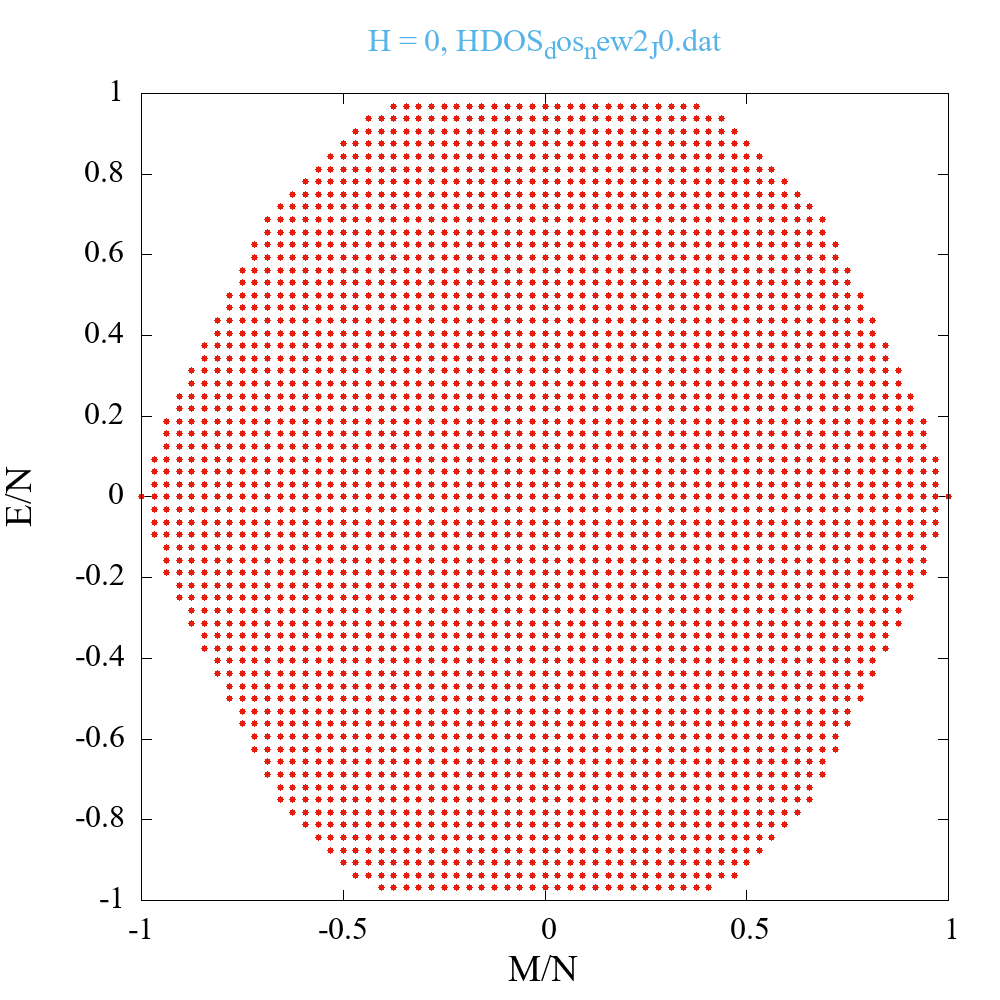
\includegraphics[width=1\linewidth]{pictures/HDOS_SI_64_J0_H0.png}
	\end{minipage}
	\hfill
	\begin{minipage}[h]{0.45\linewidth}
		\centering H=0.5
		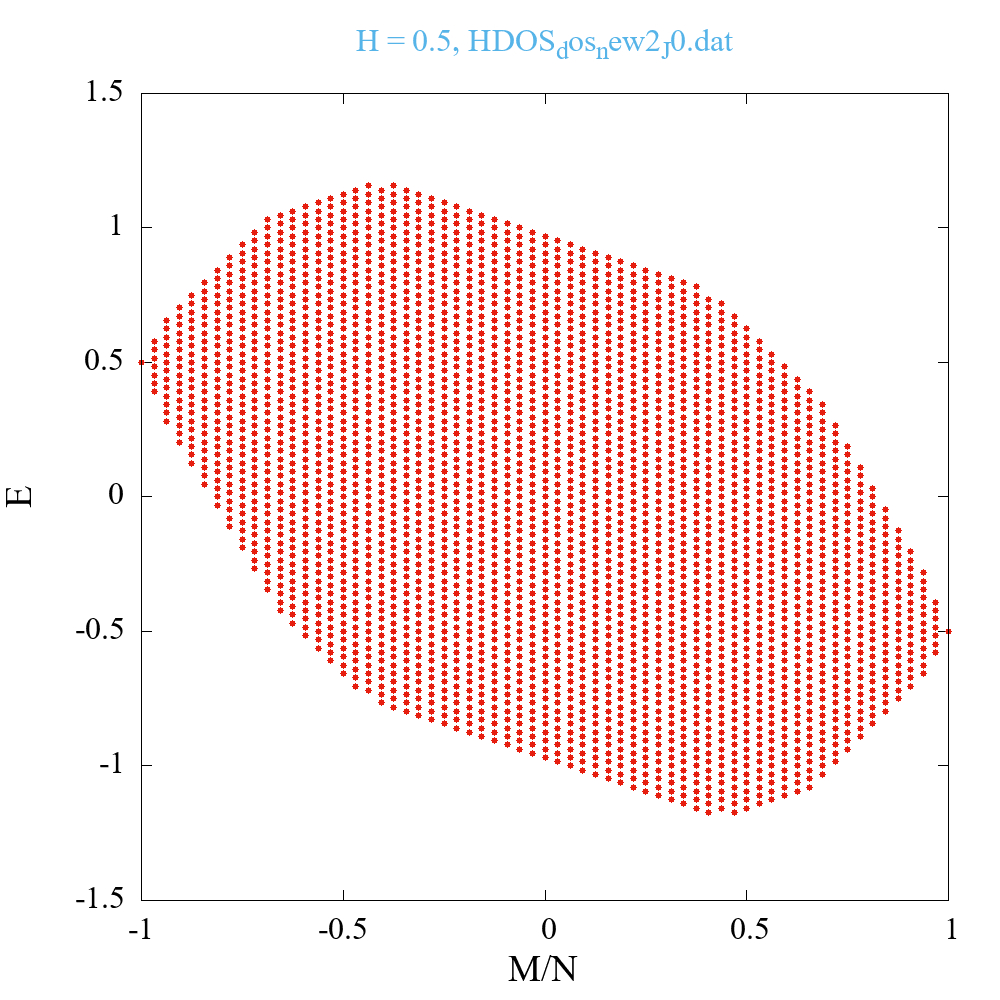
\includegraphics[width=1\linewidth]{pictures/HDOS_SI_64_J0_H0.5.png}
	\end{minipage}
	\vfill
	\begin{minipage}[h]{0.45\linewidth}
		\centering H=1
		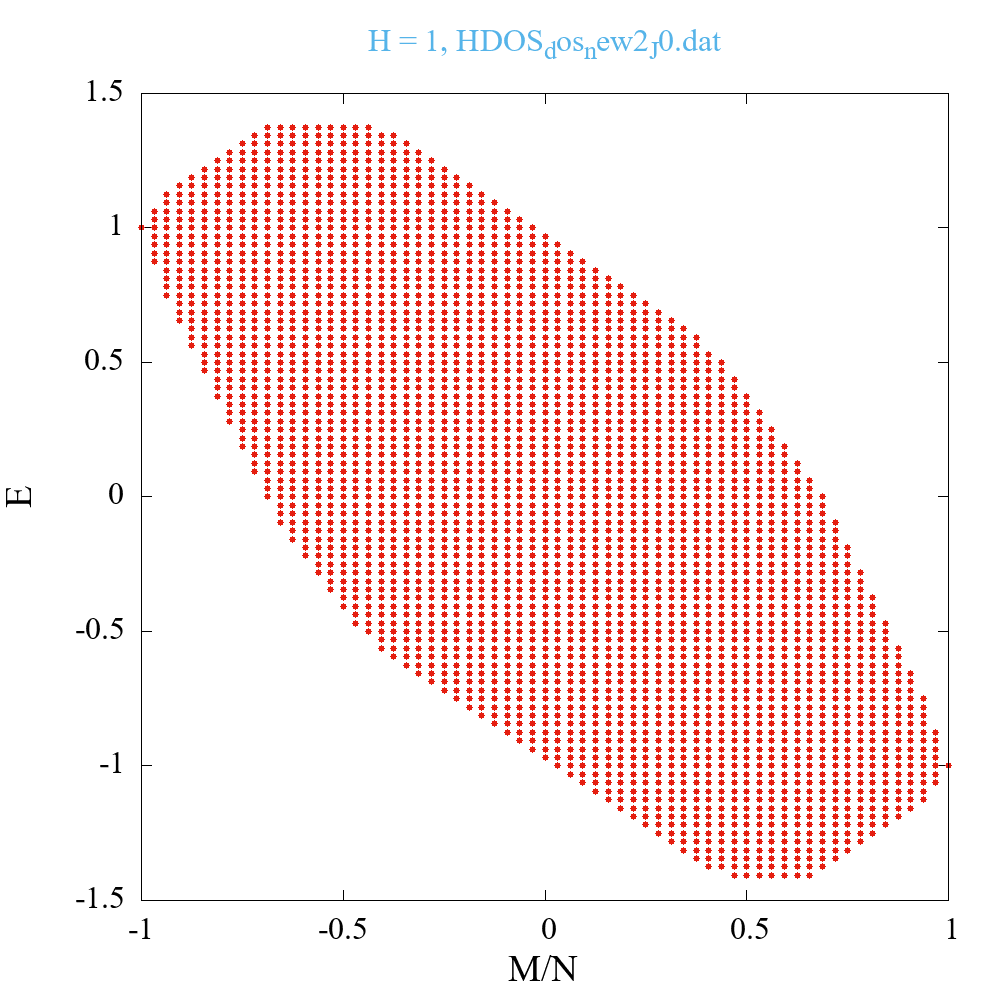
\includegraphics[width=1\linewidth]{pictures/HDOS_SI_64_J0_H1.png}
	\end{minipage}
	\hfill
	\begin{minipage}[h]{0.45\linewidth}
		\centering H=2
		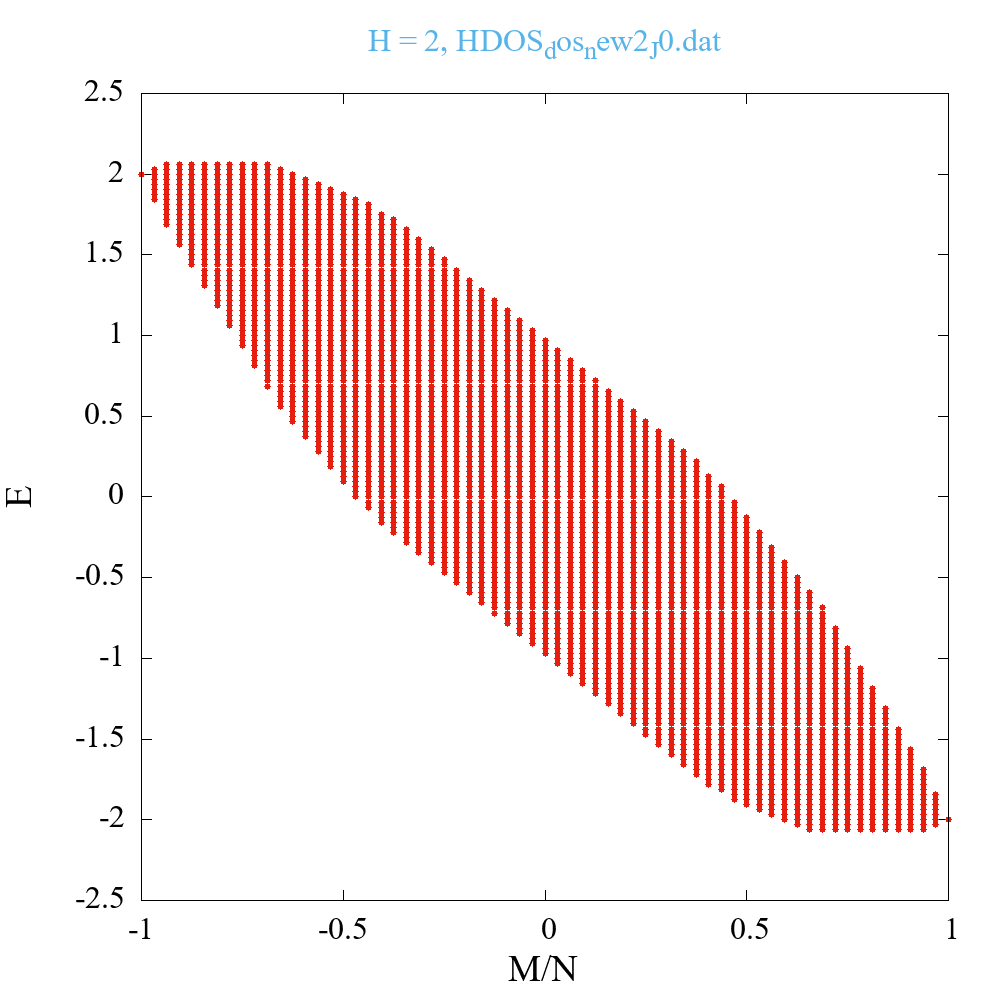
\includegraphics[width=1\linewidth]{pictures/HDOS_SI_64_J0_H2.png}
	\end{minipage}
	\vfill
	\begin{minipage}[h]{0.45\linewidth}
		\centering H=3
		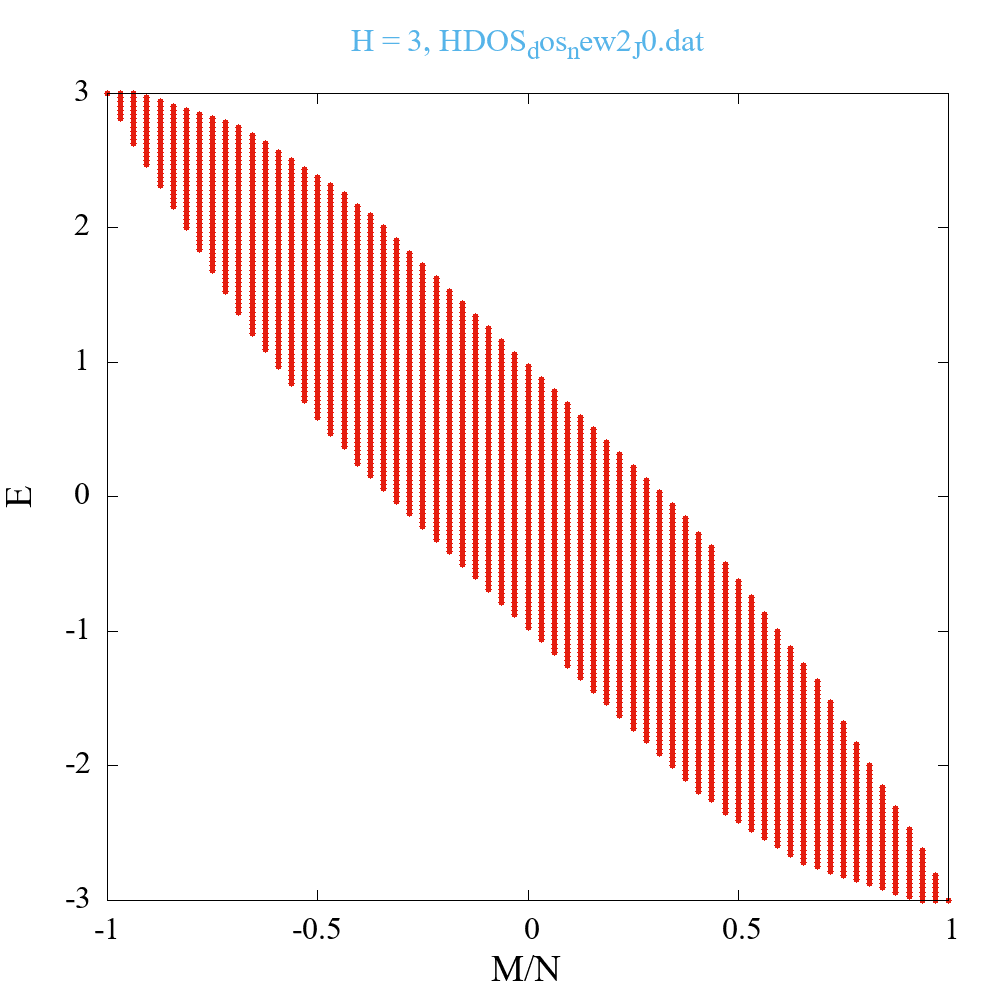
\includegraphics[width=1\linewidth]{pictures/HDOS_SI_64_J0_H3.png}
	\end{minipage}
	\caption{DOS, H=0-5, Спиновый лед, 64 спина, P+=0.5}
	\label{fig:HDOS_ice}
\end{figure}










\begin{figure}[H]
	\begin{minipage}[h]{0.45\linewidth}
		\centering H=0
		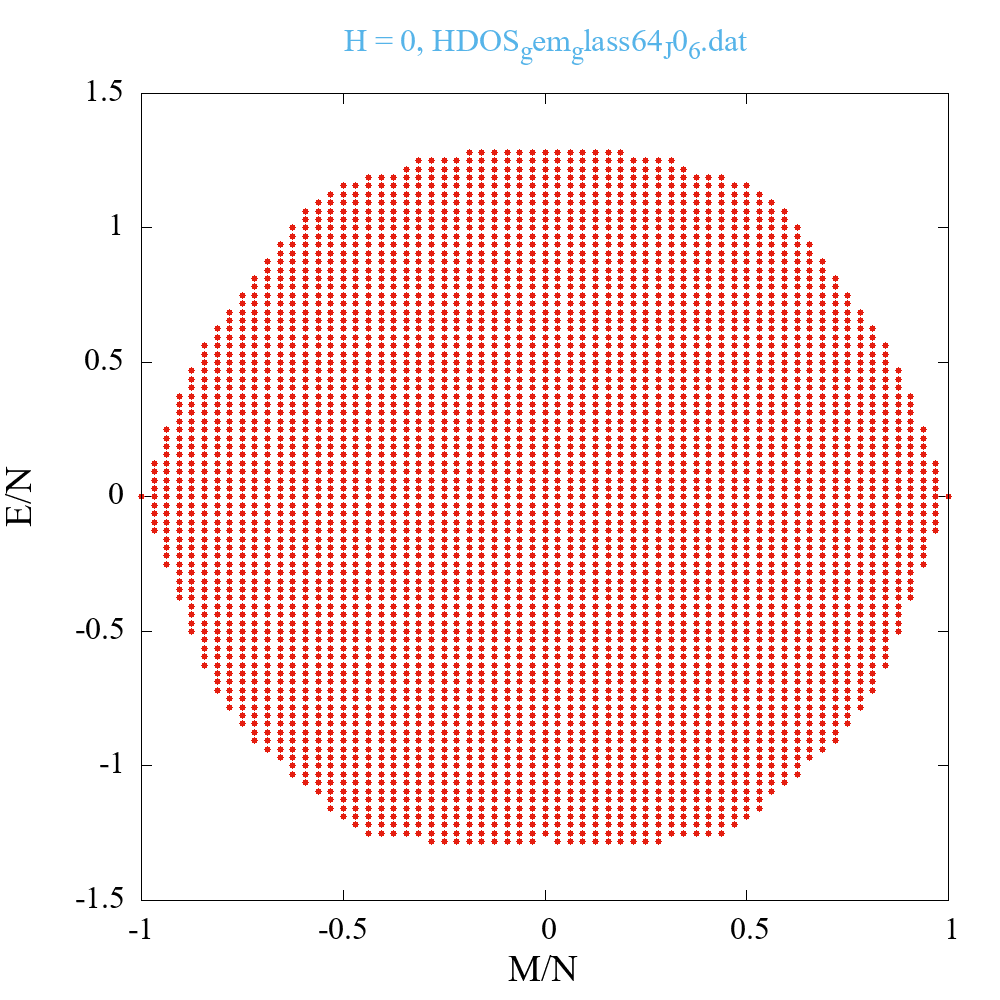
\includegraphics[width=1\linewidth]{pictures/HDOS_gem_glass64_J0_6.dat_H0.png}
	\end{minipage}
	\hfill
	\begin{minipage}[h]{0.45\linewidth}
		\centering H=0.2
		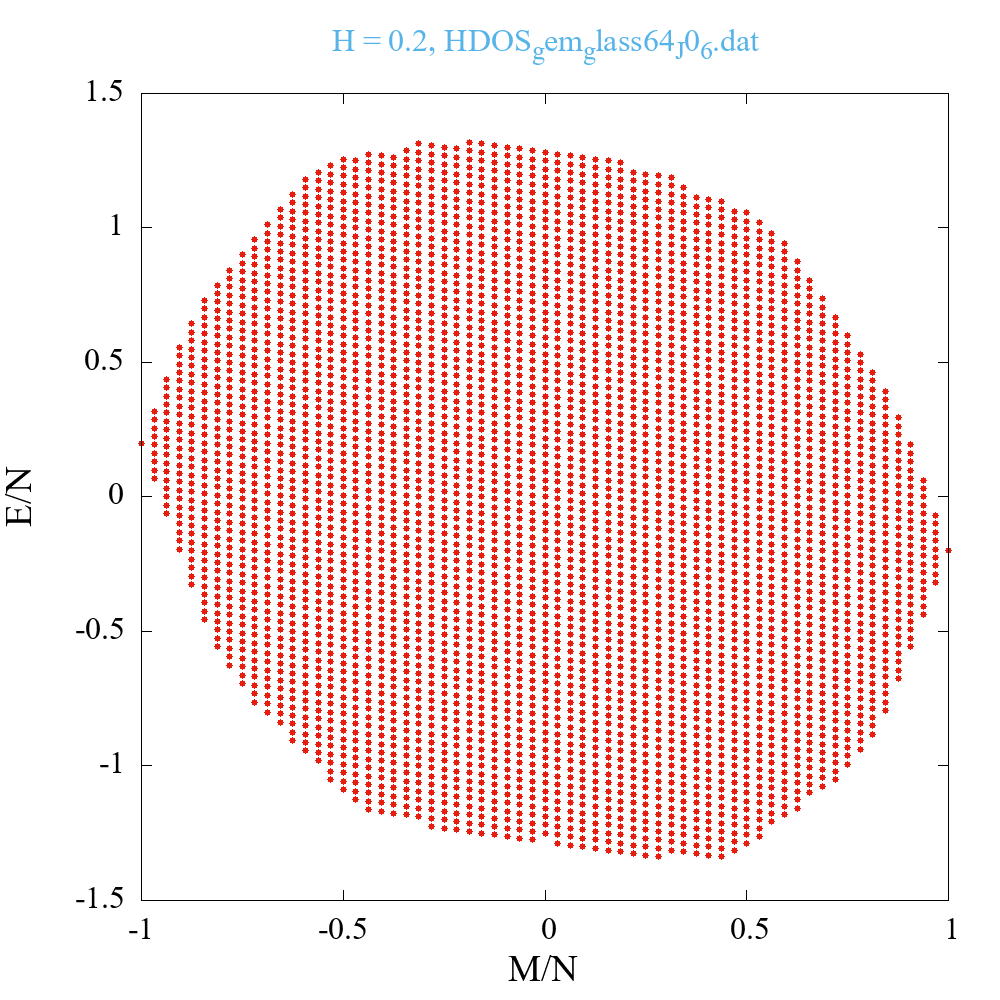
\includegraphics[width=1\linewidth]{pictures/HDOS_gem_glass64_J0_6.dat_H0.2.png}
	\end{minipage}
	\vfill
	\begin{minipage}[h]{0.45\linewidth}
		\centering H=1
		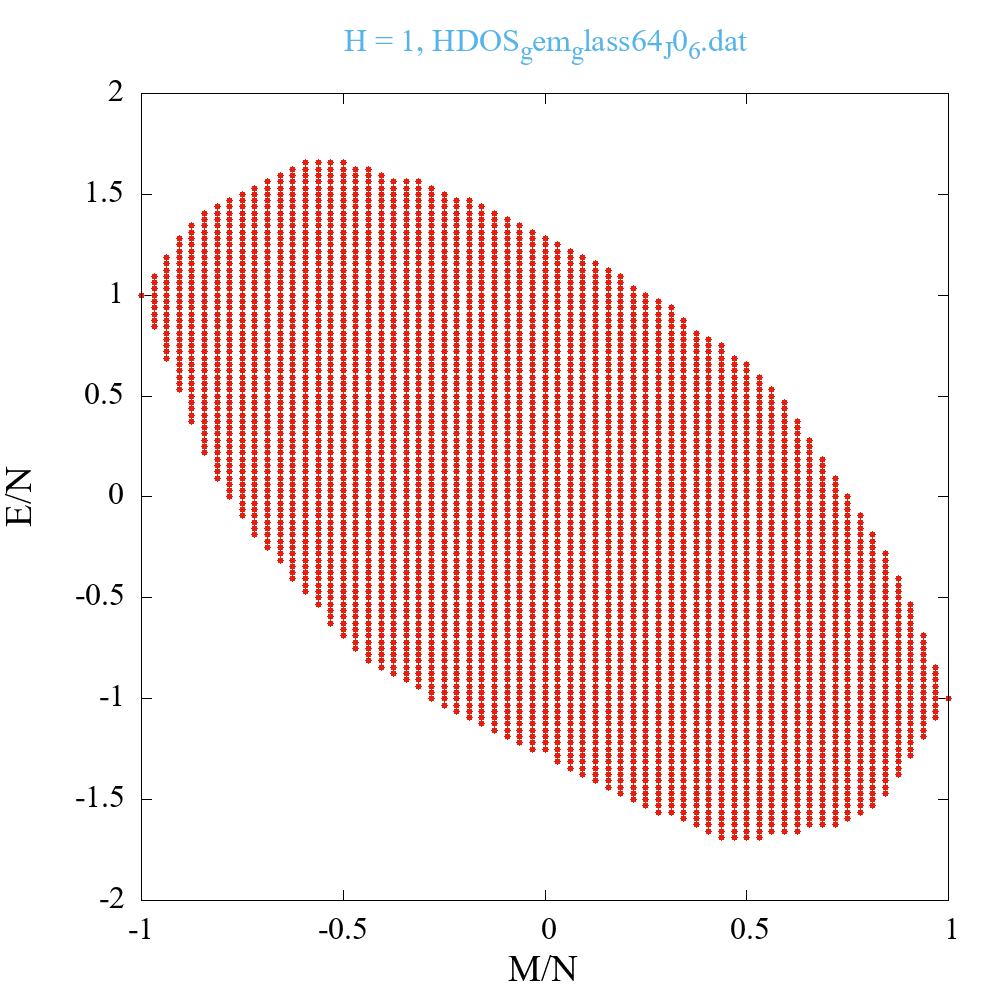
\includegraphics[width=1\linewidth]{pictures/HDOS_gem_glass64_J0_6.dat_H1.png}
	\end{minipage}
	\hfill
	\begin{minipage}[h]{0.45\linewidth}
		\centering H=1.33333
		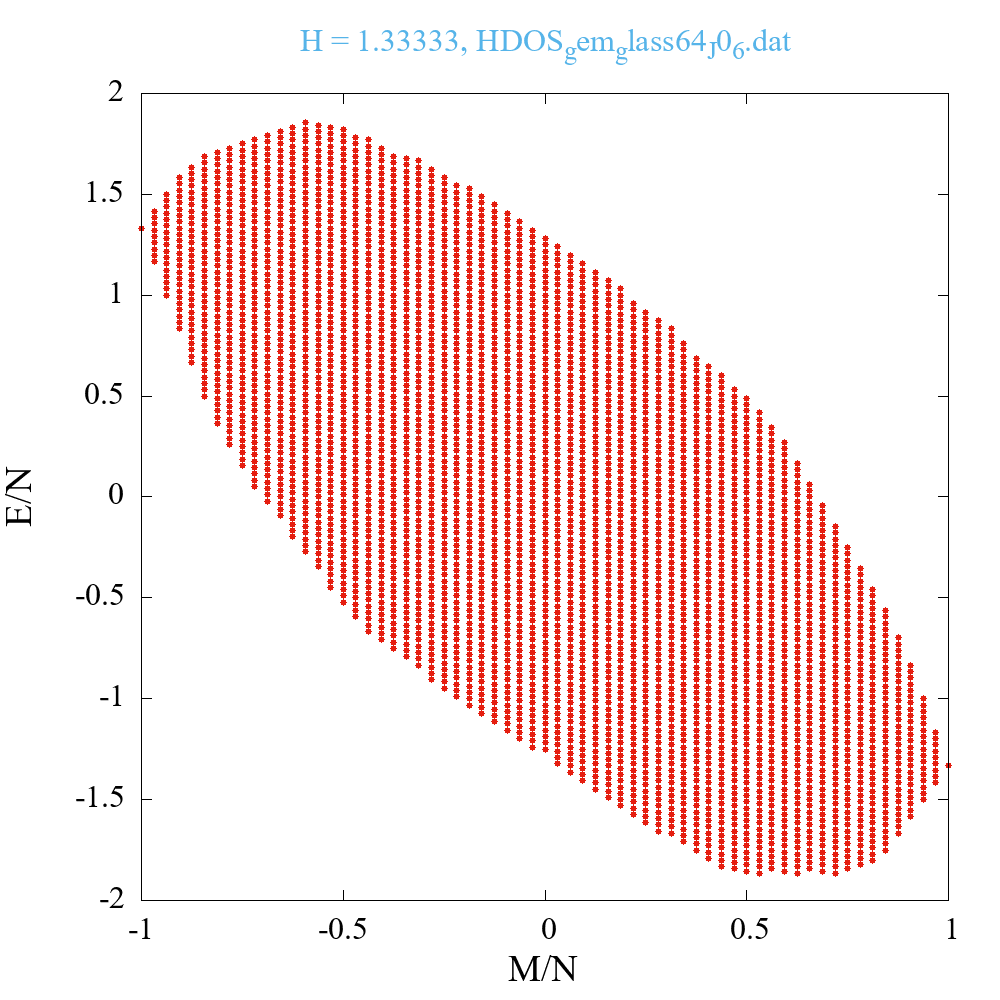
\includegraphics[width=1\linewidth]{pictures/HDOS_gem_glass64_J0_6.dat_H1.33333.png}
	\end{minipage}
	\vfill
	\begin{minipage}[h]{0.45\linewidth}
		\centering H=2
		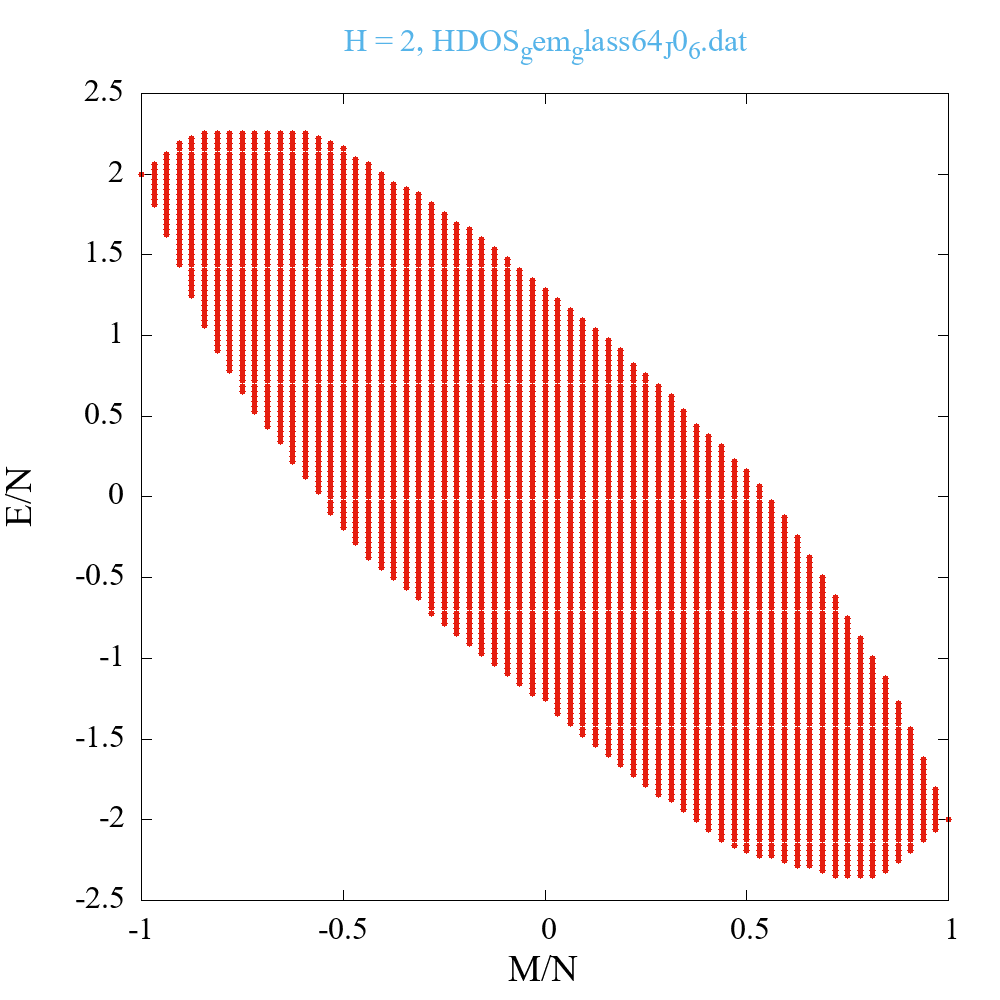
\includegraphics[width=1\linewidth]{pictures/HDOS_gem_glass64_J0_6.dat_H2.png}
	\end{minipage}
	\hfill
	\begin{minipage}[h]{0.45\linewidth}
		\centering H=3
		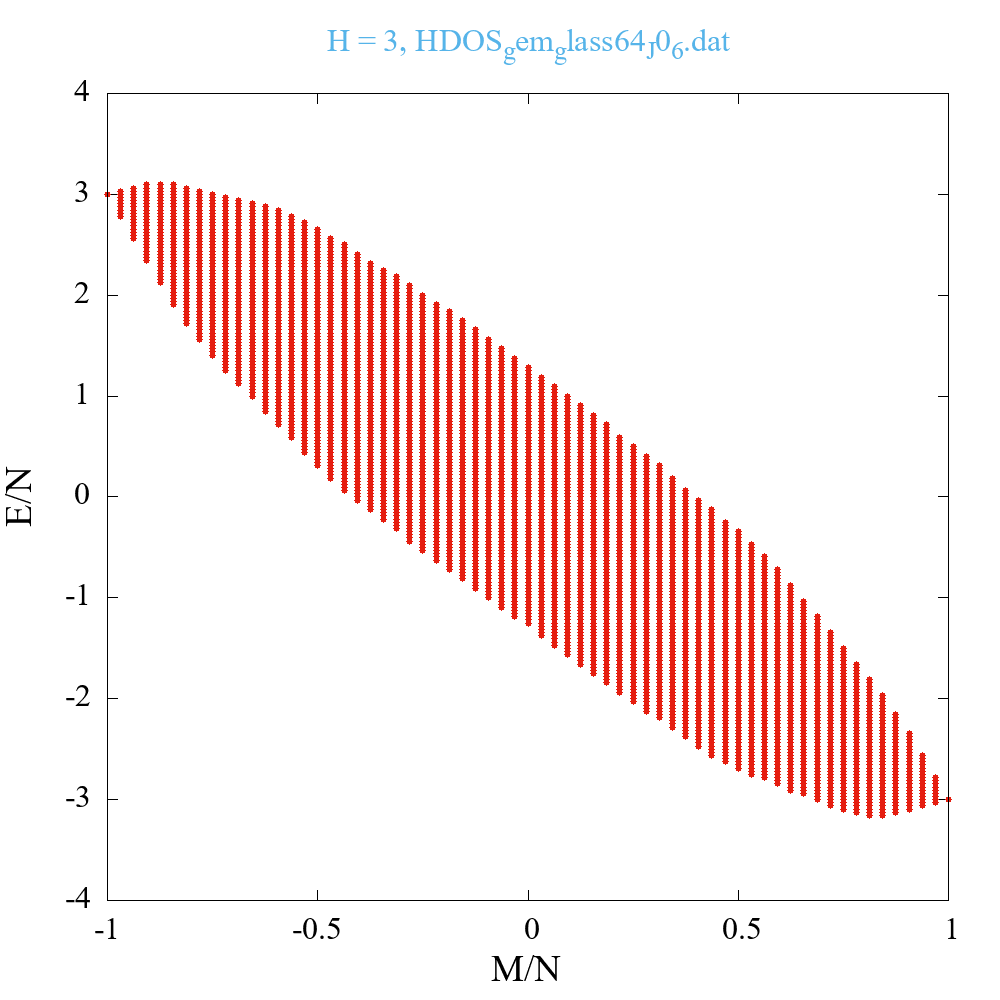
\includegraphics[width=1\linewidth]{pictures/HDOS_gem_glass64_J0_6.dat_H3.png}
	\end{minipage}
	\vfill
	\begin{minipage}[h]{0.45\linewidth}
		\centering H=4
		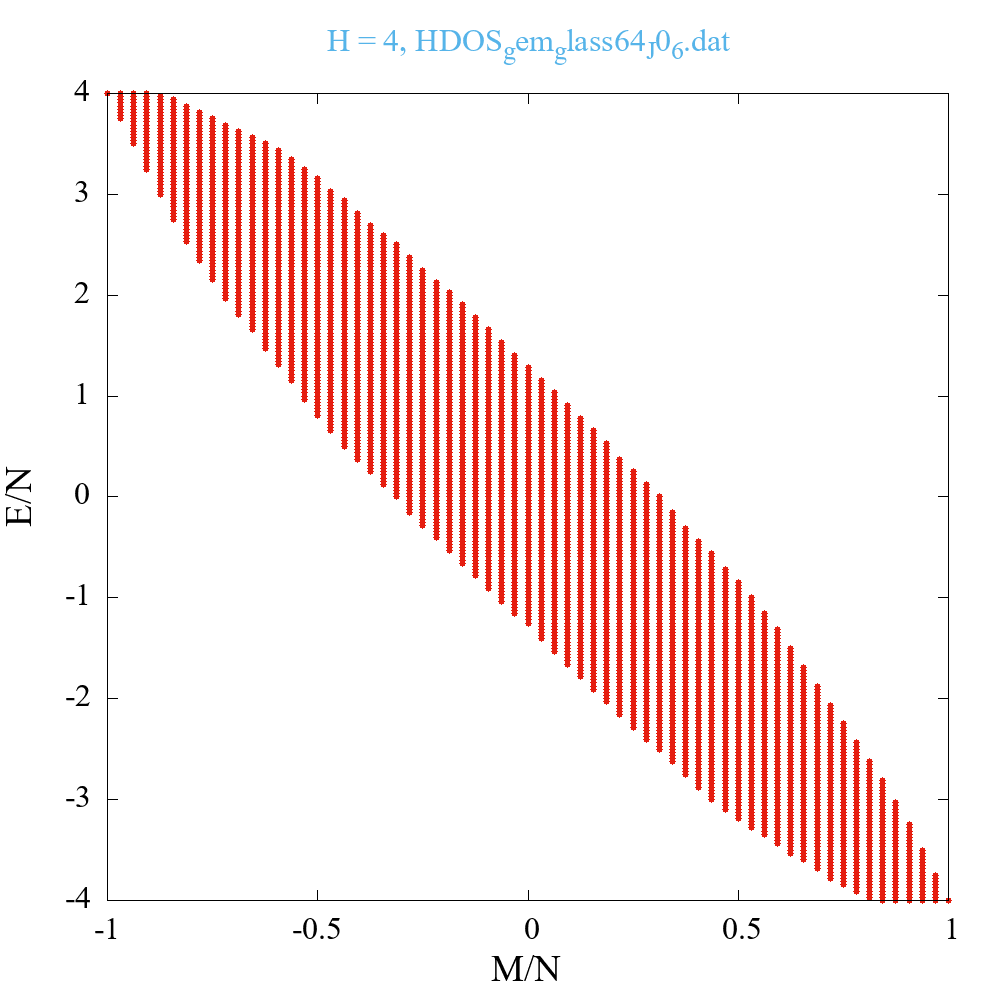
\includegraphics[width=1\linewidth]{pictures/HDOS_gem_glass64_J0_6.dat_H4.png}
	\end{minipage}
	\hfill
	\begin{minipage}[h]{0.45\linewidth}
		\centering H=5
		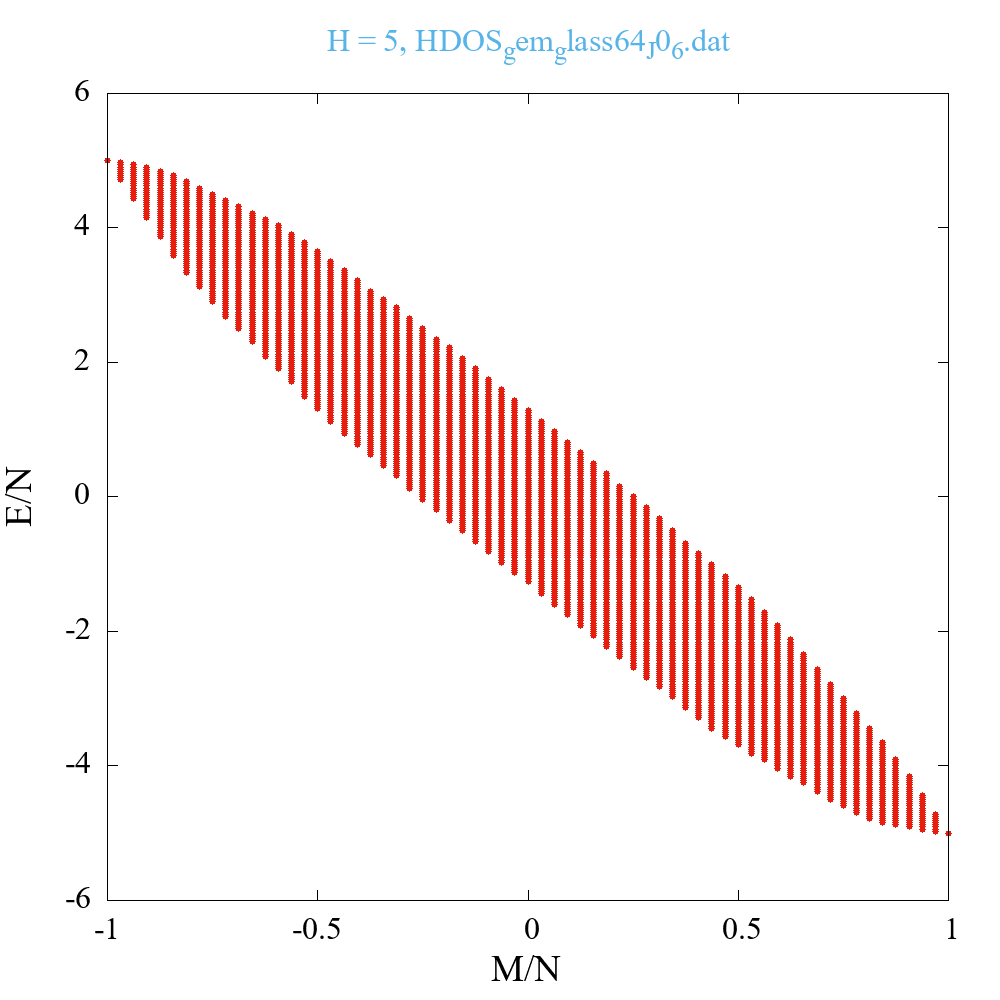
\includegraphics[width=1\linewidth]{pictures/HDOS_gem_glass64_J0_6.dat_H5.png}
	\end{minipage}
	\caption{DOS, H=0-5, Спиновое стекло, 64 спина, P+=0.5}
	\label{fig:HDOS_glass}
\end{figure}


\section{Критическая точка}

В таблице \ref{tab:lit_phase} методами представлена теоретическая точка перехода из фазы антиферромагнетика.

\begin{table}[!h]
	\begin{tabular}{|l|c|l|}
		\hline
		Method                                   & $P_{+}$                                       & Reference                                           
		\\ \hline
		Series expansion 								& ~0.099                                  & \cite{PhysRevB.19.260}    \\ \hline
	     Matching algorithm                            & 
	     0.105 $\pm 0.01$                                        & \cite{H_Freund_1989} \\ \hline
		Matching algorithm                      & 
		$0.095<p_c<0.108$                                          & \cite{BENDISCH1994139}      \\ \hline
		Exact ground states                       & 
		$0.106 \pm 0.002$                               & \cite{N.Kawashima_1997}     \\ \hline
		Ground state enumeration                             & 0.115                                          & \cite{PhysRevE.58.1502} \\ \hline
    	Exact ground states        & 
		$0.1031\pm0.0001$                                          & \cite{WANG200331}   \\ \hline
		Exact ground states   & $0.103\pm0.001$                                       & \cite{amoruso2004domain} 
		    \\ \hline
			
	\end{tabular}
	\label{tab:lit_phase}
	\caption{Критическая концентрация ферромагнитных связей}
\end{table}

В работе \cite{trukhin4855337thermodynamic} определена фазовая диаграмма при ненулевой температуре в различных полях. Однако остаётся не решенным вопрос как отделить фазу ферромагнетика и антиферромагнетика при \textbf{нулевой} температуре.

Замечено что в при определённом разбавлении антиферромагнитных или ферромагнитных связей (параметр $P_+$) в прямоугольной решетке скачки намагниченности и пики энтропии начинают появляться не только при целочисленных значениях поля, но и в дробных (рис. \ref{fig:entropy_sp_acros_AFM})

\begin{figure}[H]
	\begin{minipage}[h]{0.45\linewidth}
		\centering $P_+ = 0.05$
		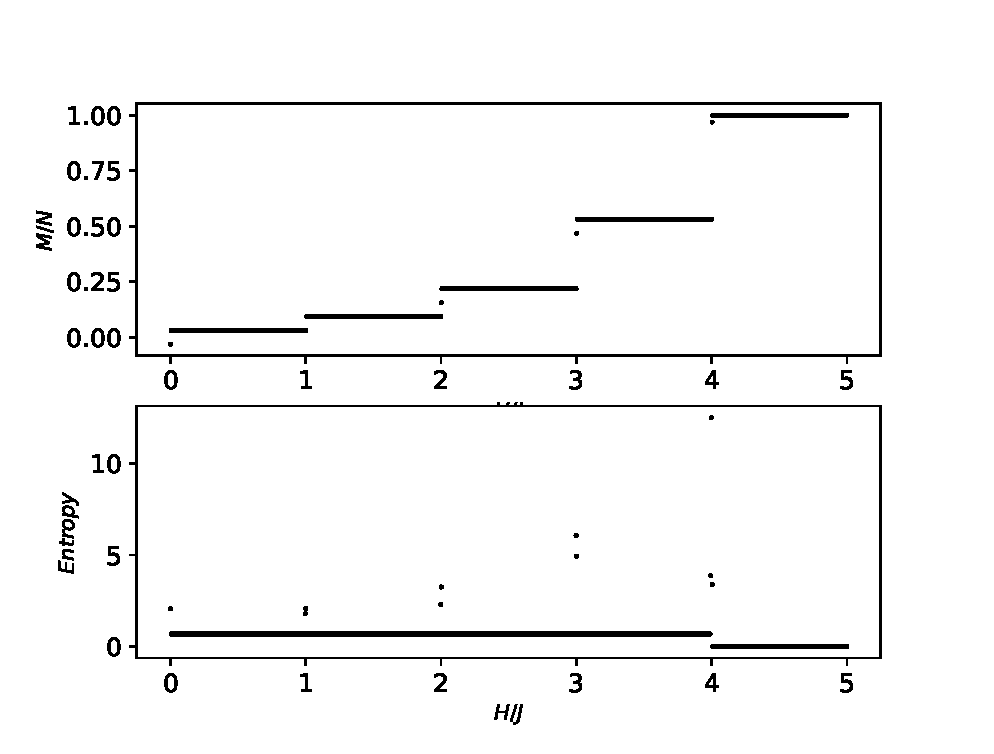
\includegraphics[width=1\linewidth]{images/Entopy_and_se_P0.05.eps}
	\end{minipage}
	\hfill
	\begin{minipage}[h]{0.45\linewidth}
		\centering $P_+ = 0.15$
		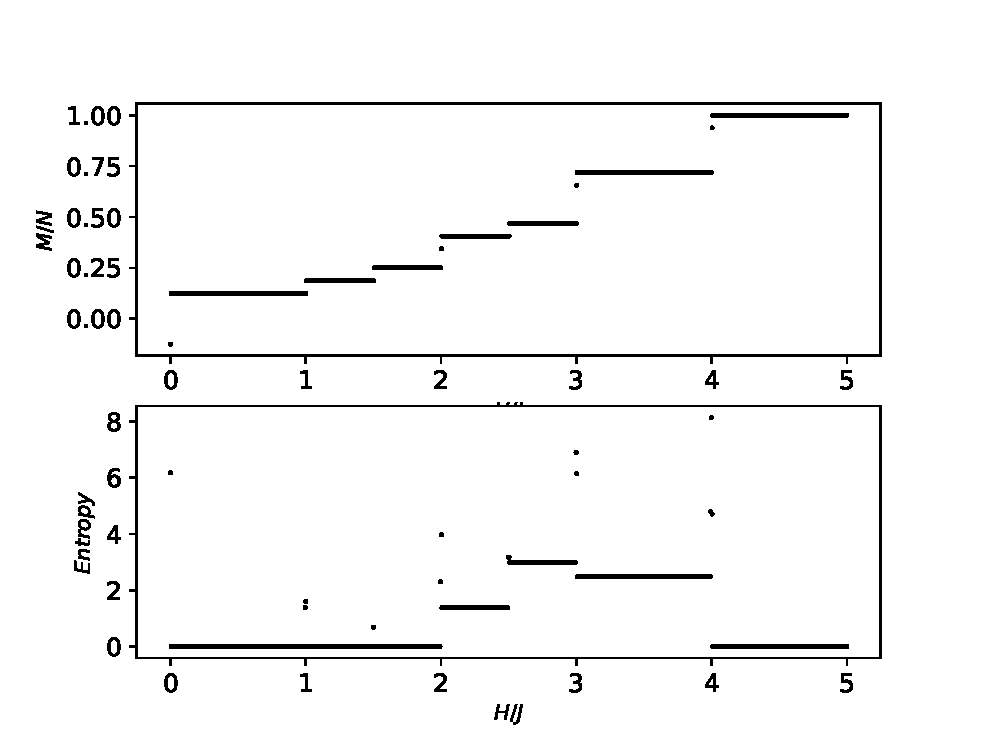
\includegraphics[width=1\linewidth]{images/Entopy_and_se_P0.15.eps}
	\end{minipage}
	\caption{Энтропия и спиновый избыток во внешнем магнитном поле}
	\label{fig:entropy_sp_acros_AFM}
\end{figure}

Проведя статистику по большой серии численных экспериментов над решетками со значением $P_+$ от 0 до 1 получена статистика представленная на рисунке \ref{fig:fractional_stairs}. На диаграмме четко отделяется фаза меньше $P_+ = 0.1$ и больше $P_+ = 0.9$.

\textbf{ОТКРЫТИЕ ПОКА ЗАКРЫВАЕТСЯ}

\begin{figure}[H]
	\centering
	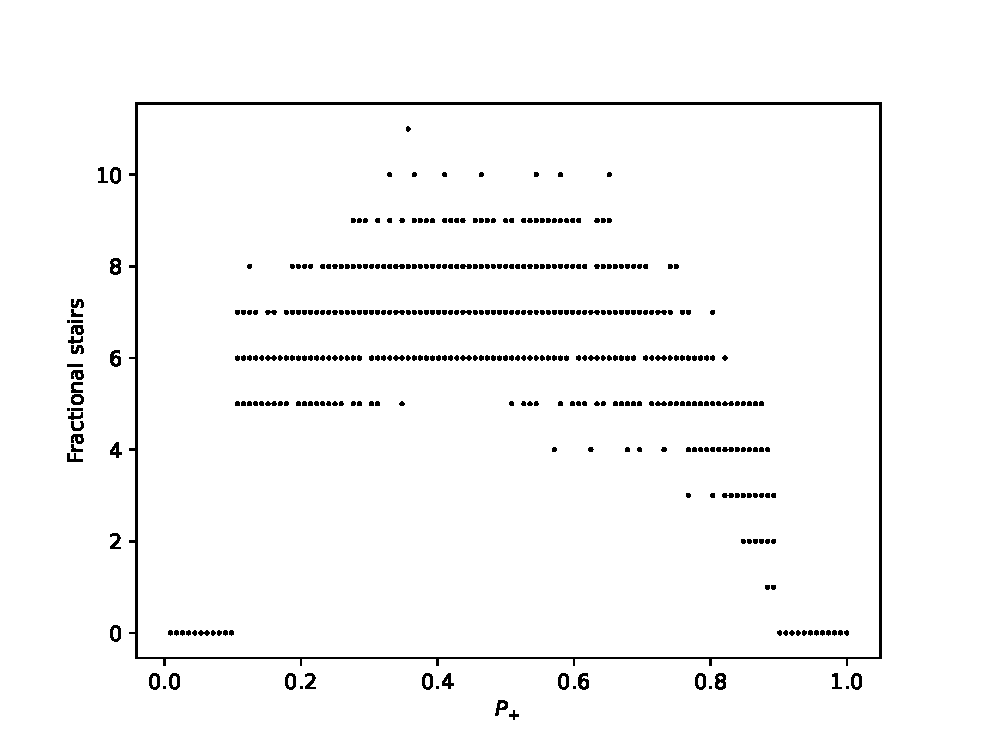
\includegraphics[width=0.8\textwidth]{images/Fractional_stairs.eps}
	\caption{Фазовая диаграмма в нулевом поле. По оси Y отложено количество скачков намагниченности в дробном значении поля}
	\label{fig:fractional_stairs}
\end{figure}

Таким образом найдены точки перехода фаз без привлечения температуры в решетку. Однако для такого отделения в качестве возбуждения была привлечена энергия из внешнего поля, что порождает новые вопросы: является ли точка перехода в нуле температур инвариантна относительно поля? А если нет то как она должна вести себя при увеличении внешнего поля? Каким образом проявится такая статистика в не прямоугольных решетках спинов?

\section{Заключение}

С помощью разработанных программ ЭВМ на основании авторского подхода, а также с помощью известных методов возможно проведение исследований основных состояний фрустрированных спиновых моделей на решетках, расчет фазовой диаграммы в отсутствии температуры, исследование возбуждений и макроскопического вырождения основного состояния в зависимости от поля, поведения спинового избытка, конфигураций основного состояния во внешнем магнитном поле для развития физики конденсированного состояния.


\section{Благодарности}

Исследование выполнено за счет гранта Российского научного фонда № 24-71-10069, https://rscf.ru/project/24-71-10069/.

The research was supported by the Russian Science Foundation grant No. 24-71-10069, https://rscf.ru/en/project/24-71-10069/.

\bibliography{mybibfile}


\end{document}